\documentclass{book}
\usepackage{a4wide}

%% possible fonts -- in order of preference
%%\usepackage{palatino}
\usepackage{bookman}
%%\usepackage{charter}
%%\usepackage{newcent}
%%\usepackage{times}
%%\usepackage{avant}
%%\usepackage{helvet}
%%\usepackage{sans}
%%\usepackage{chancery}

\usepackage[T1]{fontenc}
\usepackage{setspace}
\usepackage{ifpdf}
\usepackage{makeidx}
\usepackage{longtable}  %% page wrapping table environment
\usepackage{colortbl}   %% colors for tables
\usepackage{fancyvrb}   %% the "Verbatim" environment
\usepackage{fancyhdr}   %% custom headers and footers
\usepackage{multicol}
\usepackage{listings}   %% source code listings with syntax highlight (lstxxx commands)
\usepackage[tight]{shorttoc}   %% for generating a second table of contents, only containing chapter titles
\usepackage{bytefield}  %% for drawing protocol frames
\usepackage{paralist}   %% for compact lists
\usepackage[nottoc]{tocbibind}  %% makes Bibliography and Index show up in TOC
\settocbibname{References}

\setlength{\textwidth}{160mm}
%\setlength{\oddsidemargin}{12.5mm}
%\setlength{\evensidemargin}{12.5mm}
%\setlength{\topmargin}{0mm}
\setlength{\textheight}{220mm}
%\setlength{\parskip}{1ex}
%\setlength{\parindent}{5ex}

\renewcommand{\bottomfraction}{0.9}
\renewcommand{\topfraction}{0.9}
\renewcommand{\floatpagefraction}{0.9}

%% try to cure overfull hboxes
%% \tolerance=500

%% for navigation in dvi files, only needed by old teTeX versions
%%\usepackage{srcltx}

%% try this for spell checking: cat ess2002.tex | ispell -l -t -a | sort | uniq | more

%%
%% The following snippet changes the horizontal spacing between the number and
%% the title in the table of contents.
%%
%% http://tex.stackexchange.com/questions/33841/how-to-modify-the-space-between-the-numbers-and-text-of-sectioning-titles-in-the
%%
\makeatletter
 \renewcommand*\l@section{\@dottedtocline{1}{2em}{3em}}
 \renewcommand*\l@subsection{\@dottedtocline{2}{5em}{4em}}
\renewcommand*\l@chapter[2]{%
  \ifnum \c@tocdepth >\m@ne
    \addpenalty{-\@highpenalty}%
    \vskip 1.0em \@plus\p@
    \setlength\@tempdima{2em}%
    \begingroup
      \parindent \z@ \rightskip \@pnumwidth
      \parfillskip -\@pnumwidth
      \leavevmode \bfseries
      \advance\leftskip\@tempdima
      \hskip -\leftskip
      #1\nobreak\hfil \nobreak\hb@xt@\@pnumwidth{\hss #2}\par
      \penalty\@highpenalty
    \endgroup
  \fi}
\makeatother

%%
%% OMNeT++ logo, use as {\opp}
%%
\makeatletter
%%\DeclareRobustCommand{\omnetpp}{OM\-NeT\kern-.18em++\@}
\DeclareRobustCommand{\omnetpp}{OMNeT++\@}
\makeatother

\newcommand{\opp}{\omnetpp}

%%
%% PDF Header
%%
% note: \ifpdf now comes from the ifpdf package
%\newif\ifpdf
%\ifx\pdfoutput\undefined
%  \pdffalse
%\else
%  \pdfoutput=1
%  \pdftrue
%\fi
%% PDF-Info
\ifpdf
  \usepackage[pdftex]{graphicx}
  \usepackage[plainpages=false,linktocpage,bookmarksnumbered=true,pdftex]{hyperref}   %% automatic hyperlinking
  \pdfcompresslevel=9
  \pdfinfo{/Author (Andras Varga and others)
    /Title (INET Framework Developers Guide)
    /Subject ()
    /Keywords (INET, INETMANET, OMNeT++, manual)}
\else
  \usepackage{graphicx}
  \usepackage[plainpages=false]{hyperref}   %% automatic hyperlinking
\fi

%%
%% Draft conditional to include unfinished parts
%%
\newif\ifdraft
\draftfalse %% uncomment for final version
%\drafttrue %% uncomment for draft version

%%
%% Generate Index
%%
\makeindex


%%
%% Link colors (hyperref package)
%%
\definecolor{MyDarkBlue}{rgb}{0.16,0.16,0.5}
%% XXX the next line apparently screws up all links except in TOC! they'll be colored nicely, but won't work.
%\hypersetup{
%    colorlinks=true,
%    linkcolor=MyDarkBlue,
%    anchorcolor=MyDarkBlue,
%    citecolor=MyDarkBlue,
%    filecolor=MyDarkBlue,
%    menucolor=MyDarkBlue,
%    runcolor=MyDarkBlue,
%    urlcolor=blue,
%}

%%
%% Heading and Footer
%%
\pagestyle{fancy}
\fancyhf{}
\renewcommand{\footrulewidth}{0.5pt}
\renewcommand{\chaptermark}[1]{\markboth{#1}{}}
\lhead{INET Framework Developers Guide -- \leftmark}
\rfoot{\thepage}

%% this is used for chapter start pages
\fancypagestyle{plain}{
    \rfoot{\thepage}
}

%%
%% Use \begin{graybox}...\end{graybox} for notes
%%
\definecolor{MyGray}{rgb}{0.85,0.85,1.0}
\makeatletter\newenvironment{graybox}%
   {\begin{flushright}\begin{lrbox}{\@tempboxa}\begin{minipage}[r]{0.95\textwidth}}%
   {\end{minipage}\end{lrbox}\colorbox{MyGray}{\usebox{\@tempboxa}}\end{flushright}}%
\makeatother


\newenvironment{note}{\begin{graybox}\textbf{NOTE: }}{\end{graybox}}
\newenvironment{warning}{\begin{graybox}\textbf{WARNING: }}{\end{graybox}}
\newenvironment{caution}{\begin{graybox}\textbf{CAUTION: }}{\end{graybox}}
\newenvironment{rationale}{\begin{graybox}\textbf{Rationale: }}{\end{graybox}}
\newenvironment{important}{\begin{graybox}\textbf{IMPORTANT: }}{\end{graybox}}

%%
%% Set up listings package
%%
\lstloadlanguages{C++,make,perl,tcl,XML,R,Matlab}

%% See listings.pdf,pp20
\lstdefinelanguage{NED} {
    morekeywords={allowunconnected,bool,channel,channelinterface,connections,const,
                  default,double,extends,false,for,gates,if,import,index,inout,input,
                  int,like,module,moduleinterface,network,output,package,parameters,
                  property,simple,sizeof,string,submodules,this,true,types,volatile,
                  xml,xmldoc},
    sensitive=true,
    morecomment=[l]{//},
    morestring=[b]",
}
\lstdefinelanguage{MSG} {
    morekeywords={abstract,bool,char,class,cplusplus,double,enum,extends,false,
                  fields,int,long,message,namespace,noncobject,packet,properties,
                  readonly,short,string,struct,true,unsigned},
    sensitive=true,
    morecomment=[l]{//},
    morestring=[b]",
}
\lstdefinelanguage{inifile} {
    morekeywords={},
    sensitive=true,
    morecomment=[l]{\#},
    morestring=[b]",
}
\lstdefinelanguage{pseudocode} {
    morekeywords={if,then,else,otherwise,whenever,while},
    sensitive=true,
    morecomment=[l]{//},
    morestring=[b]",
    mathescape=true,
}

%% thick ruler on the left; also, designate backtick as LaTeX escape character
%% (e.g. \opp needs to be written as `\opp` inside listing blocks)
\lstset{
    escapechar=`,
    basicstyle=\ttfamily,
    showstringspaces=false,
    frame=leftline,
    framesep=10pt,
    framerule=3pt,
    xleftmargin=15pt
}

\definecolor{NEDRulerColor}{rgb}{0.8,1.0,0.8}  % pale green
\definecolor{MSGRulerColor}{rgb}{0.8,1.0,0.8}  % pale green
\definecolor{CPPRulerColor}{rgb}{0.8,0.8,1.0}  % pale blue
\definecolor{IniRulerColor}{rgb}{0.9,0.9,0.2}  % pale yellow
\definecolor{FileListingRulerColor}{rgb}{0.85,0.85,0.85}  % grey
%\definecolor{CommandLineRulerColor}{rgb}{0.9,0.9,0.2}
\definecolor{PseudoCodeRulerColor}{rgb}{0.0,1.0,1.0}  % cyan

%% See listings.pdf,pp39
\lstnewenvironment{ned}
    {\lstset{language=NED,rulecolor=\color{NEDRulerColor}}}
    {}
\lstnewenvironment{msg}
    {\lstset{language=MSG,rulecolor=\color{MSGRulerColor}}}
    {}
\lstnewenvironment{cpp}
    {\lstset{language=C++,rulecolor=\color{CPPRulerColor}}}
    {}
\lstnewenvironment{inifile}
    {\lstset{language=inifile,rulecolor=\color{IniRulerColor}}}
    {}
\lstnewenvironment{filelisting}
    {\lstset{language={},rulecolor=\color{FileListingRulerColor}}}
    {}
\lstnewenvironment{commandline}
    {\lstset{language={},framesep=11pt,framerule=1pt,xleftmargin=16pt}}
    {}
\lstnewenvironment{pseudocode}
    {\lstset{language=pseudocode,rulecolor=\color{PseudoCodeRulerColor}}}
    {}

%%
%% some customization
%%
\setlength{\parindent}{0pt}
\setlength{\parskip}{1ex}

%%
%% Shortcuts
%%
\newcommand{\appendixchapter}{\chapter} %% html converter needs to know which chapters are appendices

\newcommand{\tbf}{\textbf} %% bold faced text
\newcommand{\ttt}{\texttt} %% type writer font text

\newcommand{\tab}{\hspace*{5mm}} %% tabulator settings

\newcommand{\new}{$^{New!}$}
\newcommand{\changed}{$^{Changed!}$}

%% Colordefinition for table header rows (requires package colortbl)
\newcommand{\tabheadcol}{\rowcolor[gray]{0.8}}

%%
%% Module parameters list
%%
\newenvironment{params}{\begin{itemize}}{\end{itemize}}
\newcommand{\param}[2]{\item \fpar{#1}: #2}

%%
%% Function/Class/Macro/Variable/Program/Parameter/Define names
%%
%% Write the names in type writer font and do an index entry
%% Allows word wrap by automatic hyphenation
%%
%% Usage: \ffunc{take()}
%%    or: \ffunc[take()]{take(obj)}
%% the second form uses the bracketed word for the index entry
%%

%% NED type names
\newcommand{\nedtype}[2][\DefaultOpt]{\def\DefaultOpt{#2}%
  \index{#1}%
  \texttt{\hyphenchar\font=`\-\relax#2}}

%% MSG type names
\newcommand{\msgtype}[2][\DefaultOpt]{\def\DefaultOpt{#2}%
  \index{#1}%
  \texttt{\hyphenchar\font=`\-\relax#2}}

%% Function names
\newcommand{\ffunc}[2][\DefaultOpt]{\def\DefaultOpt{#2}%
  \index{#1}%
  \texttt{\hyphenchar\font=`\-\relax#2}}

%% Class names
\newcommand{\cppclass}[2][\DefaultOpt]{\def\DefaultOpt{#2}%
  \index{#1}%
  \texttt{\hyphenchar\font=`\-\relax#2}}

%% Macro names
\newcommand{\fmac}[2][\DefaultOpt]{\def\DefaultOpt{#2}%
  \index{#1}%
  \texttt{\hyphenchar\font=`\-\relax#2}}

%% Variable names
\newcommand{\fvar}[2][\DefaultOpt]{\def\DefaultOpt{#2}%
  \index{#1}%
  \texttt{\hyphenchar\font=`\-\relax#2}}

%% Program names
\newcommand{\fprog}[2][\DefaultOpt]{\def\DefaultOpt{#2}%
  \index{#1}%
  \texttt{\hyphenchar\font=`\-\relax#2}}

%% Parameter names
\newcommand{\fpar}[2][\DefaultOpt]{\def\DefaultOpt{#2}%
  \index{#1}%
  \texttt{\hyphenchar\font=`\-\relax#2}}

%% Defines
\newcommand{\fdef}[2][\DefaultOpt]{\def\DefaultOpt{#2}%
  \index{#1}%
  \texttt{\hyphenchar\font=`\-\relax#2}}

%% NED/MSG properties
\newcommand{\fprop}[2][\DefaultOpt]{\def\DefaultOpt{#2}%
  \index{#1}%
  \texttt{\hyphenchar\font=`\-\relax#2}}

%% Keywords (NED, MSG)
\newcommand{\fkeyword}[2][\DefaultOpt]{\def\DefaultOpt{#2}%
  \index{#1}%
  \textbf{\texttt{\hyphenchar\font=`\-\relax#2}}}

%% Configuration options
\newcommand{\fconfig}[2][\DefaultOpt]{\def\DefaultOpt{#2}%
  \index{#1}%
  \textbf{\texttt{\hyphenchar\font=`\-\relax#2}}}

%% File names
\newcommand{\ffilename}[2][\DefaultOpt]{\def\DefaultOpt{#2}%
  \index{#1}%
  \texttt{\hyphenchar\font=`\-\relax#2}}

%% Signals
\newcommand{\fsignal}[2][\DefaultOpt]{\def\DefaultOpt{#2}%
  \index{#1}%
  \texttt{\hyphenchar\font=`\-\relax#2}}

\newcommand{\fgate}[1]{\texttt{\hyphenchar\font=`\-\relax#1}}

%% do not number subsubsections
%\setcounter{secnumdepth}{4}

% limit the depth of TOC
\setcounter{tocdepth}{2}

%%
%% Start of document
%%
\begin{document}

%% set the image type preference
\DeclareGraphicsExtensions{.pdf,.png}

\pagestyle{empty}
\pagenumbering{roman}

%% %%\begin{figure}[htbp]
%%\begin{center}
%%\includegraphics[width=3.648in, height=0.990in]{figures/usmanFig1}
%%\end{center}
%% %%\end{figure}

%% the following {center} is a trick -- vspace does nothing if there's
%% nothing above it in the page
\begin{center}\end{center}
\vspace{16em}
\hrule
\vspace{2em}
\begin{center}
{\HUGE INET Framework}\\
\vspace{2em}
{\Huge Developer's Guide}\\
\end{center}
\vspace{2em}
\hrule

\begin{center}
\textit{\today}
\end{center}




\cleardoublepage

%%\setcounter{page}{1}
%\newpage
%%\pagenumbering{roman}

%% \shorttableofcontents{Chapters}{0}
%% \cleardoublepage

\tableofcontents
\cleardoublepage

\pagestyle{fancy}
\pagenumbering{arabic}

\chapter{Introduction}
\label{cha:introduction}


\section{What is INET Framework}

INET Framework contains IPv4, IPv6, TCP, SCTP, UDP protocol implementations,
and several application models. The framework also includes an MPLS model
with RSVP-TE and LDP signalling. Link-layer models are PPP, Ethernet and 802.11.
Static routing can be set up using network autoconfigurators, or one can use
routing protocol implementations. The INET Framework supports wireless and
mobile simulations as well.


\section{Scope of this Manual}

This manual is written for users of INET who intend to extend INET with new 
components, written in C++. This manual is accompanied by the INET Reference,
which is generated from NED and MSG files using OMNeT++'s documentation generator, 
and the documentation of the underlying C++ classes, generated from the source files 
using Doxygen. A working knowledge of OMNeT++ and the C++ language is assumed.

\ifdraft TODO
\section{Contents of this Manual}

todo...
\fi


%%% Local Variables:
%%% mode: latex
%%% TeX-master: "usman"
%%% End:


\cleardoublepage

\chapter{Getting Started}
\label{cha:gettingstarted}


\section{Contributing to INET}

Workflow:

Fork on Github.

Check out the INET project from GitHub, and import it into the OMNeT++ IDE.

Develop.

Submit pull requests.


\section{Setting Up a New INET-Based Project}

Create new project in the IDE.

Set INET as referenced project.

Set up version control (git, GitHub).

Develop.





%%% Local Variables:
%%% mode: latex
%%% TeX-master: "usman"
%%% End:


\cleardoublepage

\chapter{Node Architecture}
\label{cha:node-architecture}

\section{Addresses}

The INET Framework uses a number of C++ classes to represent various
addresses in the network. These classes support initialization and
assignment from binary and string representation of the address, and
accessing the address in both forms. (Storage is in binary form). They also
support the "unspecified" special value (and the \ffunc{isUnspecified()}
method) that corresponds to the all-zeros address.

\begin{itemize}
  \item \cppclass{MACAddress} represents a 48-bit IEEE 802 MAC address. The
    textual notation it understands and produces is hex string.

  \item \cppclass{IPv4Address} represents a 32-bit IPv4 address. It can parse
    and produce textual representations in the "dotted decimal" syntax.

  \item \cppclass{IPv6Address} represents a 128-bit IPv6 address. It can parse
    and produce address strings in the canonical (RFC 3513) syntax.

  \item \cppclass{L3Address} is conceptually a union of a \cppclass{IPv4Address}
    and \cppclass{IPv6Address}: an instance stores either an IPv4 address or an
    IPv6 address. \cppclass{L3Address} is mainly used in the transport layer and above
    to abstract away network addresses. It can be assigned from both \cppclass{IPv4Address}
    and \cppclass{IPv6Address}, and can also parse string representations of both.
    The \ffunc{getType()}, \ffunc{toIPv4()} and \ffunc{toIPv6()} methods can be used
    to access the value.
\end{itemize}

\ifdraft TODO
TODO: Resolving addresses with L3AddressResolver
\fi


\ifdraft TODO
\section{The Notification Board}

The \nedtype{NotificationBoard} module allows publish-subscribe
communication among modules within a host. Using
\nedtype{NotificationBoard}, modules can notify each other about
events such as routing table changes, interface status changes
(up/down), interface configuration changes, wireless handovers, changes in
the state of the wireless channel, mobile node position changes, etc.
\nedtype{NotificationBoard} acts as a intermediary between the module where
the events occur and modules which are interested in learning about
those events.

\nedtype{NotificationBoard} has exactly one instance within a host or
router model, and it is accessed via direct C++ method calls (not message
exchange). Modules can \textit{subscribe} to categories of changes
(e.g. ``routing table changed'' or ``radio channel became empty''). When
such a change occurs, the corresponding module (e.g. the
\nedtype{IPv4RoutingTable} or the physical layer module) will let
\nedtype{NotificationBoard} know, and it will disseminate this information
to all interested modules.

\sloppypar Notification events are grouped into \textit{categories}.
Examples of categories are: \ttt{NF\_HOSTPOSITION\_UPDATED},
\ttt{NF\_RADIOSTATE\_CHANGED}, \ttt{NF\_PP\_TX\_BEGIN},
\ttt{NF\_PP\_TX\_END}, \ttt{NF\_IPv4\_ROUTE\_ADDED},
\ttt{NF\_BEACON\_LOST}, \ttt{NF\_NODE\_FAILURE}, \ttt{NF\_NODE\_RECOVERY},
etc. Each category is identified by an integer (right now it's assigned in
the source code via an enum, in the future we'll convert to dynamic
category registration).

To trigger a notification, the client must obtain a pointer to the
\nedtype{NotificationBoard} of the given host or router (explained later),
and call its \ffunc{fireChangeNotification()} method. The notification will
be delivered to all subscribed clients immediately, inside the
\ffunc{fireChangeNotification()} call.

Clients that wish to receive notifications should implement (subclass from)
the \cppclass{INotifiable} interface, obtain a pointer to the
\nedtype{NotificationBoard}, and subscribe to the categories they are
interested in by calling the \ffunc{subscribe()} method of the
\nedtype{NotificationBoard}. Notifications will be delivered to the
\ffunc{receiveChangeNotification()} method of the client (redefined from
\cppclass{INotifiable}).

In cases when the category itself (an \ttt{int}) does not carry enough
information about the notification event, one can pass additional
information in a data class. There is no restriction on what the data class
may contain, except that it has to be subclassed from \cppclass{cObject},
and of course producers and consumers of notifications should agree on its
contents. If no extra info is needed, one can pass a \ttt{NULL} pointer in
the \ffunc{fireChangeNotification()} method.

A module which implements \cppclass{INotifiable} looks like this:

\begin{cpp}
class Foo : public cSimpleModule, public INotifiable {
    ...
    virtual void receiveChangeNotification(int category, const cObject *details) {..}
    ...
};
\end{cpp}

Note: \cppclass{cObject} was called \cppclass{cPolymorphic} in earlier versions
of OMNeT++. You may occasionally still see the latter name in source code; it
is an alias (typedef) to \cppclass{cObject}.

Obtaining a pointer to the \nedtype{NotificationBoard} module of that host/router:

\begin{cpp}
NotificationBoard *nb; // this is best made a module class member
nb = NotificationBoardAccess().get();  // best done in initialize()
\end{cpp}

TODO how to fire a notification
\fi


\section{The Interface Table}

The \nedtype{InterfaceTable} module holds one of the key data structures in
the INET Framework: information about the network interfaces in the host.
The interface table module does not send or receive messages; other modules
access it using standard C++ member function calls.

\ifdraft TODO
\subsection{Accessing the Interface Table}

If a module wants to work with the interface table, first it needs to obtain a
pointer to it. This can be done with the help of the
\cppclass{InterfaceTableAccess} utility class:

\begin{cpp}
IInterfaceTable *ift = InterfaceTableAccess().get();
\end{cpp}

\cppclass{InterfaceTableAccess} requires the interface table module to be a
direct child of the host and be called \ttt{"interfaceTable"} in order to
be able to find it. The \ffunc{get()} method never returns \ttt{NULL}: if
it cannot find the interface table module or cannot cast it to the
appropriate C++ type (\cppclass{IInterfaceTable}), it throws an exception
and stop the simulation with an error message.

For completeness, \cppclass{InterfaceTableAccess} also has a
\ffunc{getIfExists()} method which can be used if the code does not require
the presence of the interface table. This method returns \ttt{NULL} if the
interface table cannot be found.

Note that the returned C++ type is \cppclass{IInterfaceTable}; the initial
"\ttt{I}" stands for "interface". \cppclass{IInterfaceTable} is an abstract
class interface that \cppclass{InterfaceTable} implements. Using the abstract
class interface allows one to transparently replace the interface table with
another implementation, without the need for any change or even
recompilation of the INET Framework.
\fi

\subsection{Interface Entries}

Interfaces in the interface table are represented with the
\cppclass{InterfaceEntry} class. \cppclass{IInterfaceTable} provides member
functions for adding, removing, enumerating and looking up interfaces.

Interfaces have unique names and interface IDs; either can be used to look up
an interface (IDs are naturally more efficient). Interface IDs are invariant to
the addition and removal of other interfaces.

Data stored by an interface entry include:

\begin{itemize}
  \item \textit{name} and \textit{interface ID} (as described above)
  \item \textit{MTU}: Maximum Transmission Unit, e.g. 1500 on Ethernet
  \item several flags:
    \begin{itemize}
      \item \textit{down}: current state (up or down)
      \item \textit{broadcast}: whether the interface supports broadcast
      \item \textit{multicast} whether the interface supports multicast
      \item \textit{pointToPoint}: whether the interface is point-to-point link
      \item \textit{loopback}: whether the interface is a loopback interface
    \end{itemize}
  \item \textit{datarate} in bit/s
  \item \textit{link-layer address} (for now, only IEEE 802 MAC addresses are supported)
  \item \textit{network-layer gate index}: which gate of the network layer within the host the NIC is connected to
  \item \textit{host gate IDs}: the IDs of the input and output gate of the host the NIC is connected to
\end{itemize}

\tbf{Extensibility}. You have probably noticed that the above list does not
contain data such as the IPv4 or IPv6 address of the interface. Such
information is not part of \cppclass{InterfaceEntry} because we do not want
\nedtype{InterfaceTable} to depend on either the IPv4 or the IPv6 protocol
implementation; we want both to be optional, and we want
\nedtype{InterfaceTable} to be able to support possibly other network
protocols as well.

Thus, extra data items are added to \cppclass{InterfaceEntry} via
extension. Two kinds of extensions are envisioned: extension by the link
layer (i.e. the NIC), and extension by the network layer protocol:

\begin{itemize}

\item \tbf{NICs} can extend interface entries via C++ class inheritance, that is, by
simply subclassing \cppclass{InterfaceEntry} and adding extra data and
functions. This is possible because NICs create and register entries in
\nedtype{InterfaceTable}, so in their code one can just write
\ttt{new MyExtendedInterfaceEntry()} instead of \ttt{new InterfaceEntry()}.

\item \textbf{Network layer protocols} cannot add data via subclassing, so
composition has to be used. \cppclass{InterfaceEntry} contains pointers to
network-layer specific data structures. For example, there are pointers to
IPv4 specific data, and IPv6 specific data. These objects can be accessed with
the following \cppclass{InterfaceEntry} member functions: \ffunc{ipv4Data()},
\ffunc{ipv6Data()}, and \ffunc{getGenericNetworkProtocolData()}.
They return pointers of the types \cppclass{IPv4InterfaceData},
\cppclass{IPv6InterfaceData}, and \cppclass{GenericNetworkProtocolInterfaceData},
respectively. For illustration, \cppclass{IPv4InterfaceData} is installed
onto the interface entries by the \nedtype{IPv4RoutingTable} module, and it
contains data such as the IP address of the interface, the netmask, link
metric for routing, and IP multicast addresses associated with the
interface. A protocol data pointer will be \ttt{NULL} if the corresponding
network protocol is not used in the simulation; for example, in IPv4
simulations only \ffunc{ipv4Data()} will return a non-\ttt{NULL} value.


\end{itemize}


\subsection{Interface Registration}

Interfaces are registered dynamically in the initialization phase by modules
that represent network interface cards (NICs). The INET Framework makes use
of the multi-stage initialization feature of OMNeT++, and interface registration takes
place in the first stage (i.e. stage \ttt{INITSTAGE\_LINK\_LAYER}).

Example code that performs interface registration:

\begin{cpp}
void PPP::initialize(int stage)
{
    if (stage == INITSTAGE_LINK_LAYER) {
        ...
        interfaceEntry = registerInterface(datarate);
    ...
}

InterfaceEntry *PPP::registerInterface(double datarate)
{
    InterfaceEntry *e = new InterfaceEntry(this);

    // interface name: NIC module's name without special characters ([])
    e->setName(OPP_Global::stripnonalnum(getParentModule()->getFullName()).c_str());

    // data rate
    e->setDatarate(datarate);

    // generate a link-layer address to be used as interface token for IPv6
    InterfaceToken token(0, simulation.getUniqueNumber(), 64);
    e->setInterfaceToken(token);

    // set MTU from module parameter of similar name
    e->setMtu(par("mtu"));

    // capabilities
    e->setMulticast(true);
    e->setPointToPoint(true);

    // add
    IInterfaceTable *ift = findModuleFromPar<IInterfaceTable>(par("interfaceTableModule"), this);
    ift->addInterface(e);

    return e;
}
\end{cpp}


\ifdraft TODO
\subsection{Interface Change Notifications}

\nedtype{InterfaceTable} has a change notification mechanism built in, with
the granularity of interface entries.

Clients that wish to be notified when something changes in
\nedtype{InterfaceTable} can subscribe to the following notification
categories in the host's \nedtype{NotificationBoard}:

\begin{itemize}
  \item \tbf{\ttt{NF\_INTERFACE\_CREATED}}: an interface entry has been
    created and added to the interface table
  \item \tbf{\ttt{NF\_INTERFACE\_DELETED}}: an interface entry is going
    to be removed from the interface table. This is a pre-delete
    notification so that clients have access to interface data that are
    possibly needed to react to the change
% TODO hmmm -- rename the constant? also fire a post-change notification??
  \item \tbf{\ttt{NF\_INTERFACE\_CONFIG\_CHANGED}}: a configuration setting
    in an interface entry has changed (e.g. MTU or IP address)
  \item \tbf{\ttt{NF\_INTERFACE\_STATE\_CHANGED}}: a state variable in an
    interface entry has changed (e.g. the up/down flag)
\end{itemize}

In all those notifications, the data field is a pointer to the
corresponding \cppclass{InterfaceEntry} object. This is even true for
\ttt{NF\_INTERFACE\_DELETED} (which is actually a pre-delete notification).
\fi

\ifdraft TODO
\section{Initialization Stages}

Node architecture makes it necessary to use multi-stage initialization.
What happens in each stage is this:

In stage 0, interfaces register themselves in \nedtype{InterfaceTable} modules

In stage 1, routing files are read.

In stage 2, network configurators (e.g. \nedtype{FlatNetworkConfiguration})
assign addresses and set up routing tables.

In stage 3, TODO...

In stage 4, TODO...

...

The multi-stage initialization process itself is described in the OMNeT++ Manual.
\fi

\section{Communication between protocol layers}

In the INET Framework, when an upper-layer protocol wants to send a data
packet over a lower-layer protocol, the upper-layer module just sends the
message object representing the packet to the lower-layer module, which
will in turn encapsulate it and send it. The reverse process takes place
when a lower layer protocol receives a packet and sends it up after
decapsulation.

It is often necessary to convey extra information with the packet. For
example, when an application-layer module wants to send data over TCP, some
connection identifier needs to be specified for TCP. When TCP sends a
segment over IP, IP will need a destination address and possibly other
parameters like TTL. When IP sends a datagram to an Ethernet interface for
transmission, a destination MAC address must be specified. This extra
information is attached to the message object to as \textit{control info}.

Control info are small value objects, which are attached to packets
(message objects) with its \ttt{setControlInfo()} member function.
Control info only holds auxiliary information for the next protocol layer,
and is not supposed to be sent over the network to other hosts and routers.


\ifdraft TODO
\section{Publish-Subscribe Communication within Nodes}

The \nedtype{NotificationBoard} module makes it possible for several modules to
communicate in a publish-subscribe manner. For example, the radio module
(\nedtype{Ieee80211Radio}) fires a \textit{"radio state changed"} notification when
the state of the radio channel changes (from TRANSMIT to IDLE, for example),
and it will be delivered to other modules that have previously subscribed
to that notification category. The notification mechanism uses C++ functions
calls, no message sending is involved.

The notification board submodule within the host (router) must be called
\ttt{notificationBoard} for other modules to find it.
\fi

\ifdraft TODO
\section{Network interfaces}

todo...
\fi

\ifdraft TODO
\section{The wireless infrastructure}

todo...
\fi


\section{NED Conventions}

\subsection{The @node Property}

By convention, compound modules that implement network devices (hosts,
routers, switches, access points, base stations, etc.) are marked with the
\ttt{@node} NED property. As node models may themselves be hierarchical, the
\ttt{@node} property is used by protocol implementations and other simple
modules to determine which ancestor compound module represents the physical
network node they live in.

\subsection{The @labels Module Property}

The \ttt{@labels} property can be added to modules and gates, and it
allows the OMNeT++ graphical editor to provide better editing experience.
First we look at \ttt{@labels} as a module property.

\ttt{@labels(node)} has been added to all NED module types that may occur on
network level. When editing a network, the graphical editor will NED types
with \ttt{@labels(node)} to the top of the component palette, allowing the
user to find them easier.

Other labels can also be specified in the \ttt{@labels(...)} property. This
has the effect that if one module with a particular label has already been
added to the compound module being edited, other module types with the same
label are also brought to the top of the palette. For example,
\nedtype{EtherSwitch} is annotated with \ttt{@labels(node,ethernet-node)}.
When you drop an \nedtype{EtherSwitch} into a compound module, that will
bring \nedtype{EtherHost} (which is also tagged with the
\ttt{ethernet-node} label) to the top of the palette, making it easier to
find.

\begin{ned}
module EtherSwitch
{
    parameters:
        @node();
        @labels(node,ethernet-node);
        @display("i=device/switch");
    ...
}
\end{ned}

Module types that are already present in the compound module also appear in
the top part of the palette. The reason is that if you already added a
\nedtype{StandardHost}, for example, then you are likely to add more of the
same kind. Gate labels (see next section) also affect palette order: modules
which can be connected to modules already added to the compound module
will also be listed at the top of the palette. The final ordering is the
result of a scoring algorithm.


\subsection{The @labels Gate Property}

Gates can also be labelled with \ttt{@labels()}; the purpose is to make it easier
to connect modules in the editor. If you connect two modules in the editor,
the gate selection menu will list gate pairs that have a label in common.

\ifdraft TODO
screenshot
\fi

For example, when connecting hosts and routers, the editor will offer connecting
Ethernet gates with Ethernet gates, and PPP gates with PPP gates. This is the
result of gate labelling like this:

\begin{ned}
module StandardHost
{
    ...
    gates:
        inout pppg[] @labels(PPPFrame-conn);
        inout ethg[] @labels(EtherFrame-conn);
    ...
}
\end{ned}

Guidelines for choosing gate label names: For gates of modules that
implement protocols, use the C++ class name of the packet or acompanying
control info (see later) associated with the gate, whichever applies;
append \ttt{/up} or \ttt{/down} to the name of the control info class. For
gates of network nodes, use the class names of packets (frames) that travel
on the corresponding link, with the \ttt{-conn} suffix. The suffix prevents
protocol-level modules to be promoted in the graphical editor palette when
a network is edited.

Examples:

\begin{ned}
simple TCP like ITCP
{
    ...
    gates:
        input appIn[] @labels(TCPCommand/down);
        output appOut[] @labels(TCPCommand/up);
        input ipIn @labels(TCPSegment,IPv4ControlInfo/up,IPControlInfo/up);
        output ipOut @labels(TCPSegment,IPv4ControlInfo/down,IPv6ControlInfo/up);
}
\end{ned}


\begin{ned}
simple PPP
{
    ...
    gates:
        input netwIn;
        output netwOut;
        inout phys @labels(PPPFrame);
}
\end{ned}

%%% Local Variables:
%%% mode: latex
%%% TeX-master: "usman"
%%% End:


\cleardoublepage

\chapter{Point-to-Point Links}
\label{cha:ppp}


\section{Overview}

The INET Framework contains an implementation of the Point-to-Point Protocol
as described in RFC1661 with the following limitations:

\begin{itemize}
\item There are no LCP messages for link configuration,
link termination and link maintenance.
The link can be configured by setting module parameters.
\item PFC and ACFC are not supported, the PPP frame
always contains the 1-byte Address and Control fields
and a 2-byte Protocol field.
\item PPP authentication is not supported
\item Link quality monitoring protocols are not supported.
\item There are no NCP messages, the network layer protocols are
configured by other means.
\end{itemize}

The modules of the PPP model can be found in the \nedtype{inet.linklayer.ppp}
package:

\begin{description}
\item[\nedtype{PPP}] This simple module performs encapsulation
of network datagrams into PPP frames and decapsulation of
the incoming PPP frames. It can be connected to the network
layer directly or can be configured to get the outgoing messages
from an output queue. The module collects statistics about
the transmitted and dropped packages.

\item[\nedtype{PPPInterface}] is a compound module complementing
the \nedtype{PPP} module with an output queue. It implements
the \nedtype{IWiredNic} interface. Input and output hooks can be configured
for further processing of the network messages.

\end{description}

\section{PPP frames}

According to RFC1662 the PPP frames contain the following fields:

\begin{bytefield}[bitheight=2\baselineskip]{40}
\bitbox{8}{Flag \\ 01111110} &
\bitbox{8}{Address \\ 11111111} &
\bitbox{8}{Control \\ 00000011} \\
\bitbox{8}{Protocol \\ 8/16 bits} &
\bitbox{10}{Information \\ \textasteriskcentered } &
\bitbox{8}{Padding \\ \textasteriskcentered } \\
\bitbox{8}{FCS \\ 16/32 bits}
\bitbox{8}{Flag \\ 01111110 } &
\bitbox[ltb]{14}{Inter-frame Fill \\ or next Address}
\end{bytefield}

The corresponding message type in the INET framework is \msgtype{PPPFrame}.
It contains the Information field as an encapsulated \cppclass{cMessage}
object. The Flag, Address and Control fields are omitted
from \msgtype{PPPFrame} because they are constants. The FCS field is
omitted because no CRC computed during the simulation, the bit error
attribute of the \cppclass{cMessage} used instead. The Protocol
field is omitted because the protocol is determined from the class
of the encapsulated message.

The length of the PPP frame is equal to the length of the encapsulated
datagram plus 7 bytes. This computation assumes that
\begin{itemize}
\item there is no inter-octet time fill, so only one Flag sequence
needed per frame
\item padding is not applied
\item PFC and ACFC compression is not applied
\item FCS is 16 bit
\item no escaping was applied
\end{itemize}

\section{PPP module}

The PPP module receives packets from the upper layer in the \fvar{netwIn}
gate, encapsulates them into \msgtype{PPPFrame}s, and send it to the
physical layer through the \fvar{phys} gate. The \msgtype{PPPFrame}s
received from the \fvar{phys} gate are decapsulated and sent to the upper
layer immediately through the \fvar{netwOut} gate.

Incoming datagrams are waiting in a queue if the line is currently busy.
In routers, PPP relies on an external queue module (implementing
\nedtype{IOutputQueue}) to model finite buffer, implement QoS and/or RED,
and requests packets from this external queue one-by-one. The name
of this queue is given as the \fpar{queueModule} parameter.

In hosts, no such queue is used, so \nedtype{PPP} contains an internal
queue named txQueue to queue up packets wainting for transmission.
Conceptually txQueue is of inifinite size, but for better diagnostics
one can specify a hard limit in the \fpar{txQueueLimit} parameter -- if
this is exceeded, the simulation stops with an error.

The module can be used in simulations where the nodes are connected and
disconnected dinamically. If the channel between the PPP modules is down,
the messages received from the upper layer are dropped (including the messages
waiting in the queue). When the connection is restored it will
poll the queue and transmits the messages again.

The PPP module registers itself in the interface table of the node.
The \fvar{mtu} of the entry can be specified by the
\fpar{mtu} module parameter. The module checks the state of the physical link
and updates the entry in the interface table.
% FIXME: The module does not notice if the datarate of the channel changed!
%        It should update the interface entry.

\ifdraft TODO
The node containing the PPP module must also contain a
\nedtype{NofiticationBoard} component. Notifications are sent when
transmission of a new PPP frame started (\verb!NF_PP_TX_BEGIN!), finished
(\verb!NF_PP_TX_END!) or when a PPP frame received (\verb!NF_PP_RX_END!).
\fi

\ifdraft TODO
The PPP component is the source of the following signals:
\begin{itemize}
\item \tbf{txState} state of the link (0=idle,1=busy)
\item \tbf{txPkBytes} number of bytes transmitted
\item \tbf{rxPkBytesOk} number of bytes received successfully
\item \tbf{droppedPkBytesBitError} number of bytes received in erronous frames
\item \tbf{droppedPkBytesIfaceDown} number of bytes dropped because the link is down
\item \tbf{rcvdPkBytesFromHL} number of bytes received from the the upper layer
\item \tbf{passedUpPkBytes} number of bytes sent to the the upper layer
\end{itemize}

These signals are recorded as statistics (sum, count and vector), so
they can be analyzed after the simulation.
\fi

When the simulation is executed with the graphical user interface
the module displays useful statistics. If the link is operating,
the datarate and number of received, sent and dropped messages
show in the tooltip. When the link is broken, the number of dropped
messages is displayed. The state of the module is indicated by the color
of the module icon and the connection (yellow=transmitting).

\section{PPPInterface module}

The \nedtype{PPPInterface} is a compound module implementing the \nedtype{IWiredNic}
interface. It contains a \nedtype{PPP} module and a passive queue for the messages
received from the network layer.

The queue type is specified by the \fpar{queueType} parameter.
It can be set to \nedtype{NoQueue} or to a module type implementing
the \nedtype{IOutputQueue} interface. There are implementations
with QoS and RED support.

In typical use of the \nedtype{PPP} module it is augmented with other nodes
that monitor the traffic or simulate package loss and duplication.
The \nedtype{PPPInterface} module abstract that usage by adding
\nedtype{IHook} components to the network input and output of the
\nedtype{PPP} component. Any number of hook can be added by
specifying the \fpar{numOutputHooks} and \fpar{numInputHooks}
parameters and the types of the \fvar{outputHook} and \fvar{inputHook}
components. The hooks are chained in their numeric order.


%%% Local Variables:
%%% mode: latex
%%% TeX-master: "usman"
%%% End:



\cleardoublepage

% last synchronized to 'dbc28949bf4332ac86d84b95705fbea9af4f84f7'
\chapter{The Ethernet Model}
\label{cha:ethernet}

\section{Sending Ethernet Frames}

TODO tags etc

\section{Receiving Ethernet Frames}

TODO tags etc

\section{Frames}

The INET defines these frames in the \ffilename{EtherFrame.msg} file.
The models supports Ethernet II, 803.2 with LLC header, and 803.3 with LLC and SNAP headers.
The corresponding classes are:
\msgtype{EthernetIIFrame}, \msgtype{EtherFrameWithLLC} and \msgtype{EtherFrameWithSNAP}. They all class
from \msgtype{EtherFrame} which only represents the basic MAC frame with source and
destination addresses. \nedtype{EtherMAC} only deals with \msgtype{EtherFrame}s, and does not
care about the specific subclass.

Ethernet frames carry data packets as encapsulated cMessage objects.
Data packets can be of any message type (cMessage or cMessage subclass).

The model encapsulates data packets in Ethernet frames using the \ttt{encapsulate()}
method of cMessage. Encapsulate() updates the length of the Ethernet frame too,
so the model doesn't have to take care of that.

The fields of the Ethernet header are passed in a \cppclass{Ieee802Ctrl}
control structure to the LLC by the network layer.


EtherJam, EtherPadding (interframe gap), EtherPauseFrame?


\subsection{EtherLLC}

EtherFrameWithLLC

SAP registration

% TODO delete EtherLLC, because LLC without SNAP is not used with IP (no ARP,IPv6 SAP)
% TODO modify EtherEncap to handle EtherFrameWithSNAP frames too (we can not send EtherFrameWithSNAP now)

\subsubsection{\nedtype{EtherLLC} and higher layers}

The \nedtype{EtherLLC} module can serve several applications (higher layer protocols),
and dispatch data to them. Higher layers are identified by DSAP.
See section "Application registration" for more info.

\nedtype{EtherEncap} doesn't have the functionality to dispatch to different
higher layers because in practice it'll always be used with IP.

\subsubsection{Communication between LLC and Higher Layers}

Higher layers (applications or protocols) talk to the \nedtype{EtherLLC} module.

When a higher layer wants to send a packet via Ethernet, it just
passes the data packet (a cMessage or any subclass) to \nedtype{EtherLLC}.
The message kind has to be set to IEEE802CTRL\_DATA.

In general, if \nedtype{EtherLLC} receives a packet from the higher layers,
it interprets the message kind as a command. The commands include
IEEE802CTRL\_DATA (send a frame), IEEE802CTRL\_REGISTER\_DSAP (register highher layer)
IEEE802CTRL\_DEREGISTER\_DSAP (deregister higher layer) and IEEE802CTRL\_SENDPAUSE
(send PAUSE frame) -- see EtherLLC for a more complete list.

The arguments to the command are NOT inside the data packet but
in a "control info" data structure of class \cppclass{Ieee802Ctrl}, attached to
the packet. See controlInfo() method of cMessage (OMNeT++ 3.0).

For example, to send a packet to a given MAC address and protocol
identifier, the application sets the data packet's message kind
to ETH\_DATA ("please send this data packet" command),
fills in the \nedtype{Ieee802Ctrl} structure with the destination MAC address and
the protocol identifier, adds the control info to the message, then sends
the packet to \nedtype{EtherLLC}.

When the command doesn't involve a data packet (e.g.
IEEE802CTRL\_(DE)REGISTER\_DSAP, IEEE802CTRL\_SENDPAUSE), a dummy packet
(empty cMessage) is used.

\subsubsection{Rationale}

The alternative of the above communications would be:

\begin{itemize}
  \item adding the parameters such as destination address into the data
    packet. This would be a poor solution since it would make the
    higher layers specific to the Ethernet model.
  \item encapsulating a data packet into an \textit{interface packet} which
    contains the destination address and other parameters. The
    disadvantages of this approach is the overhead associated with
    creating and destroying the interface packets.
\end{itemize}

Using a control structure is more efficient than the interface packet
approach, because the control structure can be created once inside
the higher layer and be reused for every packet.

It may also appear to be more intuitive in Tkenv because one can observe
data packets travelling between the higher layer and Ethernet
modules -- as opposed to "interface" packets.


\subsubsection{EtherLLC: SAP Registration}

The Ethernet model supports multiple applications or higher layer
protocols.

So that data arriving from the network can be dispatched to the
correct applications (higher layer protocols), applications
have to register themselves in \nedtype{EtherLLC}. The registration
is done with the IEEE802CTRL\_REGISTER\_DSAP command
(see section "Communication between LLC and higher layers")
which associates a SAP with the LLC port. Different applications
have to connect to different ports of \nedtype{EtherLLC}.

The ETHERCTRL\_REGISTER\_DSAP/IEEE802CTRL\_DEREGISTER\_DSAP commands use only the
dsap field in the \cppclass{Ieee802Ctrl} structure.

%%% Local Variables:
%%% mode: latex
%%% TeX-master: "usman"
%%% End:

\cleardoublepage

\chapter{The Physical Environment}
\label{cha:environment}

\section{Overview}

Wireless networks are heavily affected by the physical environment, and the
requirements for today's ubiquitous wireless communication devices are
increasingly demanding. Cellular networks serve densely populated urban
areas, wireless LANs need to be able to cover large buildings with several
offices, low-power wireless sensors must tolerate noisy industrial
environments, batteries need to remain operational under various external
conditions, and so on.

The propagation of radio signals, the movement of communicating agents,
battery exhaustion, etc., depend on the surrounding physical environment.
For example, signals can be absorbed by objects, can pass through objects,
can be refracted by surfaces, can be reflected from surfaces, or battery
nominal capacity might depend on external temperature. These effects cannot
be ignored in high-fidelity simulations.

In order to help the modeling process, the model of the physical
environment is separated from the rest of the simulation models. The main
goal of the physical environment model is to describe buildings, walls,
vegetation, terrain, weather, and other physical objects and conditions
that might have effects on radio signal propagation, movement, batteries,
etc. This separation makes the model reusable by all other simulation
models that depend on these circumstances.

The following sections provide a brief overview of the physical environment
model.

\section{The Physical Environment Model}

The physical environment is represented in an INET simulation by a
\nedtype{PhysicalEnvironment} module. This module normally has one instance
in the network, and acts as a database that other parts of the simulation
can query at runtime.

\section{Global Physical Properties}

The physical environment model stores the following global
properties:

\begin{itemize}
  \item \textit{space limits}: global bounds for the 3-dimensional space
  \item \textit{temperature}: global parameter for temperature-dependent models
\end{itemize}

Space limits are useful for limiting the propagation and reflection of
radio signals, to constrain movement of communicating agents, and for
detecting incorrectly positioned physical objects.

Temperature can be useful for modeling batteries, as it affects the
maximum capacity, internal resistance, self-discharge and other properties
of real-life electrochemical energy storage devices.

\section{Physical Objects}

The most important aspect of the physical environment is the objects which
are present in it. For example, simulating an indoor Wifi scenario may need
to model walls, floors, ceilings, doors, windows, furniture, and similar
objects, because they all affect signal propagation.

Objects are located in space, and have shapes and materials. The INET
physical layer infrastructure supports basic shapes and homogeneous
materials, which simplifies description and still allows for a reasonable
approximation of reality. Physical objects in INET have the following
properties:

\begin{itemize}
  \item \textit{shape}: describes the 3-dimensional shape of the object,
    independent of its position and orientation
  \item \textit{position}: determines where the object is located in the 3-dimensional space
  \item \textit{orientation}: determines how the object is rotated relative to its
    default orientation
  \item \textit{material}: describes material-specific physical properties
  \item \textit{graphical properties}: provides parameters for better visualization
\end{itemize}

Physical objects in INET are stationary, they cannot change their position
or orientation over time.

Since the shape of the physical objects might be quite diverse, the model
is designed to be extensible with new shapes. Concave shapes are not yet
supported, such shapes can be represented by splitting them up into smaller,
convex parts. The current implementation provides the following shapes:

\begin{itemize}
  \item \textit{sphere}: specified by a radius
  \item \textit{cuboid}: specified by a length, a width, and a height
  \item \textit{prism}: specified by a 2-dimensional polygon base and a height
  \item \textit{polyhedron}: specified by the convex hull of a set of
    3-dimensional vertices
\end{itemize}

\section{Visualization}

The \nedtype{PhysicalEnvironment} module is capable is visualizing the objects on the
user interface. Rendering makes use of the following graphical object properties:

\begin{itemize}
  \item \textit{line width}: affects surface outline
  \item \textit{line color}: affects surface outline
  \item \textit{fill color}: affects surface fill
  \item \textit{opacity}: affects surface outline and fill
  \item \textit{tags}: allows filtering objects on the graphical user interface
\end{itemize}

The projection of 3D objects to the 2D canvas can be parameterized with an
arbitrary view angle. The default view angle is the Z axis (i.e. top view).
The view angle can also be changed during runtime, by changing the
appropriate module parameter.

The projection mechanism can be accessed by other models (e.g. mobility
models) for their own visualizations.

\section{Specifying Physical Objects}

Physical objects are defined for the \nedtype{PhysicalEnvironment} module
in an XML document. The document format allows one to define physical objects
together with their properties, and one can also define shapes and materials
that are shared (i.e. referenced) by several objects.

The following example shows some shapes, materials and objects defined in XML:

\begin{verbatim}
<environment>
  <!-- shapes and materials -->
  <shape id="1" type="sphere" radius="10"/>
  <shape id="2" type="cuboid" size="20 30 40"/>
  <shape id="3" type="prism" height="100"
         points="0 0 100 0 100 100 0 100"/>
  <shape id="4" type="polyhedron"
         points="0 0 0 100 0 0 100 100 0 0 100 0 ..."/>
  <material id="1" resistivity="100"
         relativePermittivity="4.5" relativePermeability="1"/>

  <!-- an object that uses a previously defined shape and material -->
  <object position="min 100 200 0" orientation="45 -30 0"
          shape="1" material="1"
          line-color="0 0 0" fill-color="112 128 144" opacity="0.5"/>

  <!-- an object defined with an in-line shape -->
  <object position="min 100 200 0" orientation="45 -30 0"
          shape="cuboid 20 30 40" material="concrete"
          line-color="0 0 0" fill-color="112 128 144" tags="Building"/>
</environment>
\end{verbatim}

For more details, please refer to the documentation of the
\nedtype{PhysicalEnvironment} module.

\section{Data Structure}

In order to model the physical environment in detail, a scenario might contain
several thousands or even more physical objects. Simulation models might
need to query these objects quite often. For example, when the physical layer
computes obstacle loss for a transmission, it needs to find the obstructing
physical objects for each receiver. This requires computing the intersection
between physical objects and the path traveled by the radio signal.

To speed up the computation of intersections, INET stores physical objects
in a highly efficient data structure, which currently can be one of the
following:

\begin{itemize}
  \item \nedtype{GridObjectCache}: organizes objects into a 3D spatial grid with
    a configurable constant cell size, where cells contain the objects that
    intersect with them
  \item \nedtype{BVHObjectCache}: organizes objects into a 3D tree, where
    leaves contain a configurable number of closely positioned objects.
    (This data structure is similar to quadtree and octree, but is designed for
    storing finite-sized objects.)
\end{itemize}

The physical environment model uses \nedtype{GridObjectCache} by default.

%%% Local Variables:
%%% mode: latex
%%% TeX-master: "usman"
%%% End:


\cleardoublepage

\chapter{Modeling Power Consumption}
\label{cha:power}

\section{Overview}

Modeling power consumption becomes more and more important with the increasing
number of embedded devices and the upcoming Internet of Things. Mobile personal
medical devices, large scale wireless environment monitoring devices, electric
vehicles, solar panels, low-power wireless sensors, etc. require paying special
attention to power consumption. The high fidelity simulation of power
consumption allows designing power sensitive routing protocols, MAC protocols,
physical layers, etc. which in turn results in more energy efficient devices.

In order to help the modeling process the power model is separated from other
simulation models. This separation makes the model extensible and it also allows
easy experimentation with alternative implementations. In a nutshell the power
model consists of the following components:

\begin{itemize}
  \item energy consumption models
  \item energy generation models
  \item temporary energy storage models
\end{itemize}

The power model elements fall into two categories, abbreviated with \ttt{Ep}
and \ttt{Cc} as part of their names: 

\begin{itemize}
  \item \ttt{Ep} models are simpler, and deal with energy and power quantities.
  \item \ttt{Cc} models are more realistic, and deal with charge, current, and voltage quantities.
\end{itemize}

The following sections provide a brief overview of the power model.

\section{Energy Consumer Models}

Energy consumer models describe the energy consumption of devices over time. 
For example, a transceiver consumes energy when it transmits or
receives signals, a CPU consumes energy when the network protocol routes
packets, and a display consumes energy when it's turned on.

In INET, an energy consumer model is an OMNeT++ simple module that implements
the energy consumption of software processes or hardware devices over time.
Its main purpose is to provide the power or current consumption for the
current simulation time. Most often energy consumers are included as
submodules in the compound module of the hardware devices or software
components.

INET provides only a few built-in energy consumer models:

\begin{itemize}
        \item \nedtype{AlternatingEpEnergyGenerator} is a trivial energy/power based statistical energy consumer model example.
        \item \nedtype{StateBasedEpEnergyConsumer} is a transceiver energy consumer model based on the radio mode and transmission/reception states.
\end{itemize}

In order to simulate power consumption in a wireless network, the energy
consumer model type must be configured for the transceivers. The following
example demonstrates how to configure the power consumption parameters for
a transceiver energy consumer model:

\inisnippet{EnergyConsumerConfigurationExample}{Energy consumer configuration example}


\section{Energy Generator Models}

Energy generator models describe the energy generation of devices over time. 
A solar panel, for example, produces energy based on time, the panel's 
position on the globe, its orientation towards the sun and the actual weather 
conditions. Energy generators connect to an energy storage that absorbs the 
generated energy. 

In INET, an energy generator model is an OMNeT++ simple module implementing
the energy generation of a hardware device using a physical phenomena over
time. Its main purpose is to provide the power or current generation for
the current simulation time. Most often energy generation models are
included as submodules in network nodes.

INET provides only one trivial energy/power based statistical energy
generator model called \nedtype{AlternatingEpEnergyGenerator}. The following
example shows how to configure its power generation parameters:

\inisnippet{EnergyGeneratorConfigurationExample}{Energy generator configuration example}

\section{Energy Storage Models}

Electronic devices which are not connected to external power source must contain 
some component to store energy. For example, an electrochemical battery in a
mobile phone provides energy for its display, its CPU, and its communication
devices. It might also absorb energy produced by a solar installed on its
display, or by a portable charger plugged into the wall socket.

In INET, an energy storage model is an OMNeT++ simple module which models
the physical phenomena that is used to store energy produced by generators
and provide energy for consumers. Its main purpose is to compute the amount
of available energy or charge at the current simulation time. It maintains
a set of connected energy consumers and energy generators, their respective
total power consumption and total power generation.

INET contains a few built-in energy storage models:

\begin{itemize}
        \item \nedtype{IdealEpEnergyStorage} is an idealistic model with infinite energy capacity and infinite power flow.
        \item \nedtype{SimpleEpEnergyStorage} is a non-trivial model integrating the difference between the total consumed power and the total generated power over time.
        \item \nedtype{SimpleCcBattery} is a more realistic charge/current based battery model using a charge independent ideal voltage source and internal resistance.
\end{itemize}

The following example shows how to configure a simple energy storage model:

\inisnippet{EnergyStorageConfigurationExample}{Energy storage configuration example}

\section{Energy Management Models}

% Why energy management models are needed?
% The energy management models monitors an energy storage, estimates its state, and controls the consumers and generators to protect the energy storage from operating outside its safe operating area.

\nedtype{SimpleEpEnergyManagement}

\inisnippet{EnergyManagementConfigurationExample}{Energy management configuration example}



%%% Local Variables:
%%% mode: latex
%%% TeX-master: "usman"
%%% End:


\cleardoublepage

\chapter{The Physical Layer}
\label{cha:physicallayer}

\section{Overview}

Wireless network interfaces contain a radio model component, which is
responsible for modeling the physical layer (PHY).\footnote{Wired network interfaces
could similarly contain an explicit PHY model. The reason they do not is that
wired links normally have very low error rates and simple observable behavior,
and there is usually not much to be gained from modeling the physical layer in detail.}
The radio model describes the physical device that is capable of transmitting
and receiving signals on the medium. 

Conceptually, a radio model relies on several sub-models:

\begin{itemize}
  \item antenna model
  \item transmitter model 
  \item receiver model 
  \item error model (as part of the receiver model)
  \item energy consumption model 
\end{itemize}

The antenna model is shared between the transmitter model and the receiver model.
The separation of the transmitter model and the receiver model allows 
asymmetric configurations. The energy consumer model is optional, and 
it is only used when the simulation of energy consumption is necessary.




\section{Generic Radio}

In INET, radio models implement the \nedtype{IRadio} module interface. 
A generic, often used implementation of \nedtype{IRadio} is the 
\nedtype{Radio} NED type. \nedtype{Radio} is an active compound module, 
that is, it has an associated C++ class that encapsulates the computations.

\nedtype{Radio} contains its antenna, transmitter, receiver and energy
consumer models as submodules with parametric types:

\begin{ned}
antenna: <antennaType> like IAntenna;
transmitter: <transmitterType> like ITransmitter;
receiver: <receiverType> like IReceiver;
energyConsumer: <energyConsumerType> like IEnergyConsumer 
    if energyConsumerType != "";
\end{ned}

The following sections describe the parts of the radio model.

\section{Components of a Radio}

\subsection{Antenna Models}

The antenna model describes the effects of the physical device which converts
electric signals into radio waves, and vice versa. This model captures the
antenna characteristics that heavily affect the quality of the communication
channel. For example, various antenna shapes, antenna size and geometry, antenna
arrays, and antenna orientation causes different directional or frequency
selectivity.

The antenna model provides a position and an orientation using a mobility model
that defaults to the mobility of the node. The main purpose of this model is to
compute the antenna gain based on the specific antenna characteristics and the
direction of the signal. The signal direction is computed by the medium from the
position and the orientation of the transmitter and the receiver. The following
list provides some examples:

\begin{itemize}
  \item \nedtype{IsotropicAntenna}: antenna gain is exactly 1 in any direction
  \item \nedtype{ConstantGainAntenna}: antenna gain is a constant determined by
    a parameter
  \item \nedtype{DipoleAntenna}: antenna gain depends on the direction according
    to the dipole antenna characteristics
  \item \nedtype{InterpolatingAntenna}: antenna gain is computed by linear
    interpolation according to a table indexed by the direction angles
\end{itemize}

\subsection{Transmitter Models}

The transmitter model describes the physical process which converts packets into
electric signals. In other words, this model converts an L2 frame into a signal
that is transmitted on the medium. The conversion process and the representation
of the signal depends on the level of detail and the physical characteristics
of the implemented protocol.

There are two main levels of detail (or modeling depths):
 
\begin{itemize}
\item In the \textit{flat model}, the transmitter model skips the symbol domain 
and the sample domain representations, and it directly creates the analog domain 
representation. The bit domain representation is reduced to the bit length of 
the packet, and the actual bits are ignored.

\item In the \textit{layered model}, the conversion process involves various 
processing steps such as packet serialization, forward error correction encoding, 
scrambling, interleaving, and modulation. This transmitter model requires 
significantly more computation, but it produces accurate bit domain, 
symbol domain, and sample domain representations.
\end{itemize}

Some of the transmitter types available in INET:

\begin{itemize}
  \item \nedtype{UnitDiskTransmitter}
  \item \nedtype{ApskScalarTransmitter}
  \item \nedtype{ApskDimensionalTransmitter}
  \item \nedtype{ApskLayeredTransmitter}
  \item \nedtype{Ieee80211ScalarTransmitter}
  \item \nedtype{Ieee80211DimensionalTransmitter}
\end{itemize}




\subsection{Receiver Models}

The receiver model describes the physical process which converts electric
signals into packets. In other words, this model converts a reception, along
with an interference computed by the medium model, into a MAC packet and a
reception indication.

For a packet to be received successfully, reception must be \textit{possible}
(based on reception power, bandwidth, modulation scheme and other characteristics),
it must be \textit{attempted} (i.e. the receiver must synchronize itself on
the preamble and start receiving), and it must be \textit{successful} 
(as determined by the error model and the simulated part of the signal decoding).

In the \textit{flat model}, the receiver model skips the sample domain, the symbol domain,
and the bit domain representations, and it directly creates the packet domain
representation by copying the packet from the transmission. It uses the error
model to decide whether the reception is successful.

In the \textit{layered model}, the conversion process involves various processing steps
such as demodulation, descrambling, deinterleaving, forward error correction
decoding, and deserialization. This reception model requires much more
computation than the flat model, but it produces accurate sample domain, 
symbol domain, and bit domain representations.

Some of the receiver types available in INET:

\begin{itemize}
  \item \nedtype{UnitDiskReceiver}
  \item \nedtype{ApskScalarReceiver}
  \item \nedtype{ApskDimensionalReceiver}
  \item \nedtype{ApskLayeredReceiver}
  \item \nedtype{Ieee80211ScalarReceiver}
  \item \nedtype{Ieee80211DimensionalReceiver}
\end{itemize}


\subsection{Error Models}

Determining reception errors is a crucial part of the reception process.
There are often several different statistical error models in the literature
even for a particular physical layer. In order to support this diversity, the
error model is a separate replaceable component of the receiver. 

The error model describes how the signal to noise ratio affects the amount of
errors at the receiver. The main purpose of this model is to determine whether
the received packet has errors or not. It also computes various physical
layer indications for higher layers such as packet error rate, bit error rate,
and symbol error rate. For the layered reception model it needs to compute the
erroneous bits, symbols, or samples depending on the lowest simulated physical
domain where the real decoding starts. The error model is optional (if omitted,
all receptions are considered successful.)

The following list provides some examples:

\begin{itemize}
  \item \nedtype{StochasticErrorModel}: simplistic error model with constant
    symbol/bit/packet error rates as parameters; suitable for testing. 
  \item \nedtype{ApskErrorModel} 
  \item \nedtype{Ieee80211NistErrorModel}, \nedtype{Ieee80211YansErrorModel}, 
    \nedtype{Ieee80211BerTable\-Error\-Model}: various error models for IEEE 802.11
    network interfaces.
\end{itemize}

\subsection{Power Consumption Models}

A substantial part of the energy consumption of communication devices comes from
transmitting and receiving signals. The energy consumer model describes how the
radio consumes energy depending on its activity. This model is optional (if
omitted, energy consumption is ignored.) 

The following list provides some examples:

\begin{itemize}
  \item \nedtype{StateBasedEpEnergyConsumer}: power consumption is
    determined by the radio state (a combination of radio mode, 
    transmitter state and receiver state), and specified in 
    parameters like \fpar{receiverIdlePowerConsumption} and 
    \fpar{receiverReceivingDataPowerConsumption}, in watts.
  \item \nedtype{StateBasedCcEnergyConsumer}: similar to the previous
    one, but consumption is given in amp\`eres.
\end{itemize}

\section{Layered Radio Models}

In layered radio models, the transmitter and receiver models are split
to several stages to allow more fine-grained modeling. 

For transmission, processing steps such as packet serialization, 
forward error correction (FEC) encoding, scrambling, interleaving, and 
modulation are explicitly modeled. Reception involves the inverse
operations: demodulation, descrambling, deinterleaving, 
FEC decoding, and deserialization.

In layered radio models, these processing steps are encapsulated
in four stages, represented as four submodules in both the 
transmitter and receiver model: 

\begin{enumerate}
  \item \textit{Encoding and Decoding} describe how the packet domain 
    signal representation is converted into the bit domain, and vice versa.
  \item \textit{Modulation and Demodulation} describe how the bit domain
    signal representation is converted into the symbol domain, and vice versa.
  \item \textit{Pulse Shaping and Pulse Filtering} describe how the 
    symbol domain signal representation is converted into the sample domain, 
    and vice versa.
  \item \textit{Digital Analog and Analog Digital Conversion} describe 
    how the sample domain signal representation is converted into the 
    analog domain, and vice versa.
\end{enumerate}

In layered radio transmitters and receivers such as \nedtype{ApskLayeredTransmitter}
and \nedtype{ApskLayeredReceiver}, these submodules have parametric
types to make them replaceable. This provides immense freedom for 
experimentation.

\section{Notable Radio Models}

The \nedtype{Radio} module has several specialized versions derived
from it, where certain submodule types and parameters are set to fixed values.
This section describes some of the frequently used ones.

The radio can be replaced in wireless network interfaces by setting the
\fpar{radioType} parameter, like in the following ini file fragment.
  
\begin{inifile}
**.wlan[*].radioType = "UnitDiskRadio"
\end{inifile}

However, be aware that not all MAC protocols can be used with all radio models,
and that some radio models require a matching transmission medium module. 

\subsection{UnitDiskRadio}

\nedtype{UnitDiskRadio} provides a very simple but fast and predictable 
physical layer model. It is the implementation (with some extensions)
of the \textit{Unit Disk Graph} model, which is widely used 
for the study of wireless ad-hoc networks.
\nedtype{UnitDiskRadio} is applicable if network nodes need 
to have a finite communication range, but physical effects 
of signal propagation are to be ignored.

\nedtype{UnitDiskRadio} allows three radii to be given as parameters,
instead of the usual one: communication range, interference range, and
detection range. One can also turn off interference modeling 
(meaning that signals colliding at a receiver will all be received 
correctly), which is sometimes a useful abstraction.

\nedtype{UnitDiskRadio} needs to be used together with a special physical
medium model, \nedtype{UnitDiskRadioMedium}.

The following ini file fragment shows an example configuration.

\begin{inifile}
*.radioMediumType = "UnitDiskRadioMedium"
*.host[*].wlan[*].radioType = "UnitDiskRadio"
*.host[*].wlan[*].radio.transmitter.bitrate = 2Mbps
*.host[*].wlan[*].radio.transmitter.preambleDuration = 0s
*.host[*].wlan[*].radio.transmitter.headerLength = 100b
*.host[*].wlan[*].radio.transmitter.communicationRange = 100m
*.host[*].wlan[*].radio.transmitter.interferenceRange = 0m    
*.host[*].wlan[*].radio.transmitter.detectionRange = 0m
*.host[*].wlan[*].radio.receiver.ignoreInterference = true
\end{inifile}

As a side note, if modeling full connectivity and ignoring 
interference is required, then \nedtype{ShortcutInterface} 
provides an even simpler and faster alternative.

\subsection{APSK Radio}

APSK radio models provide a hypothetical radio that simulates 
one of the well-known ASP, PSK and QAM modulations. 
(APSK stands for Amplitude and Phase-Shift Keying.)

APSK radio has scalar/dimensional, and flat/layered variants.
The flat variants, \nedtype{ApskScalarRadio} and \nedtype{ApskDimensionalRadio}
model frame transmissons in the selected modulation scheme
but without utilizing other techniques such as forward error 
correction (FEC), interleaving, spreading, etc. These radios
require matching medium models, \nedtype{ApskScalarRadioMedium}
and \nedtype{ApskDimensionalRadioMedium}.

The layered versions, \nedtype{ApskLayeredScalarRadio} 
and \nedtype{ApskLayeredDimensionalRadio} can not only
model the processing steps missing from their simpler counterparts,
they also feature configurable level of detail: the transmitter
and receiver modules have \fpar{levelOfDetail} parameters that 
control which domains are actually simulated.
These radio models must be used in conjuction with
\nedtype{ApskLayeredScalarRadioMedium} and 
\nedtype{ApskLayeredDimensionalRadioMedium}, respectively.



%%% Local Variables:
%%% mode: latex
%%% TeX-master: "usman"
%%% End:


\cleardoublepage

\chapter{The 802.11 Model}
\label{cha:80211}

% https://summit.omnetpp.org/archive/2016/assets/pdf/OMNET-2016-Session_9-02-Presentation.pdf

\section{Overview}

This chapter provides an overview of the IEEE 802.11 model for the INET Framework.

An IEEE 802.11 interface (NIC) comes in several flavours, differring
in their role (ad-hoc station, infrastructure mode station, or
access point) and their level of detail:

\begin{enumerate}
 \item \nedtype{Ieee80211Interface}: a generic (configurable) NIC
 \item \nedtype{Ieee80211NicAdhoc}: for ad-hoc mode
 \item \nedtype{Ieee80211NicAP}, \nedtype{Ieee80211NicAPSimplified}: for use in an access point
 \item \nedtype{Ieee80211NicSTA}, \nedtype{Ieee80211NicSTASimplified}: for use in an
   infrastructure-mode station
\end{enumerate}

NICs consist of four layers, which are the following (in top-down order):

\begin{enumerate}
  \item agent
  \item management
  \item MAC
  \item physical layer (radio)
\end{enumerate}

The following sections examine the above components.

\section{MAC}

The \nedtype{Ieee80211Mac} module type represents the IEEE 802.11 MAC.
The implementation is entirely based on the standard IEEE 802.11™-2012 Part 11:
Wireless LAN Medium Access Control (MAC) and Physical Layer (PHY)
Specifications.

\nedtype{Ieee80211Mac} performs transmission of frames according
to the CSMA/CA protocol. It receives data and management frames from
the upper layers, and transmits them.

The \nedtype{Ieee80211Mac} was designed to be modular to facilitate experimenting
with new policies, features and algorithms within the MAC layer. Users can
easily replace individual components with their own implementations. Policies,
which most likely to be experimented with, are extracted into their own modules.

The model has the following replaceable built-in policies:

\begin{itemize}
  \item ACK policy
  \item RTS/CTS policy
  \item Originator and recipient block ACK agreement policies
  \item MSDU aggregation policy
  \item Fragmentation policy
\end{itemize}

The new model also separates the following components:

\begin{itemize}
  \item Coordination functions
  \item Channel access methods
  \item MAC data services
  \item Aggregation and deaggregation
  \item Fragmentation and defragmentation
  \item Block ACK agreements and reordering
  \item Frame exchange sequences
  \item Duplicate removal
  \item Rate selection
  \item Rate control
  \item Protection mechanisms
  \item Recovery procedure
  \item Contention
  \item Frame queues
  \item TX/RX
\end{itemize}

\section{Physical Layer}

\textit{The physical layer} modules (\nedtype{Ieee80211Radio}) deal with modelling
transmission and reception of frames. They model the characteristics of
the radio channel, and determine if a frame was received correctly
(that is, it did not suffer bit errors due to low signal power or
interference in the radio channel). Frames received correctly are passed
up to the MAC. The implementation of these modules is based on the
Mobility Framework.

\section{Management}

\textit{The management layer} performs encapsulation and decapsulation of data packets
for the MAC, and exchanges management frames via the MAC with its peer
management entities in other STAs and APs. Beacon, Probe Request/Response,
Authentication, Association Request/Response etc frames are generated
and interpreted by management entities, and transmitted/received via
the MAC layer. During scanning, it is the management entity that periodically
switches channels, and collects information from received beacons and
probe responses.

The management layer has several implementations which differ in their role
(STA/AP/ad-hoc) and level of detail: \nedtype{Ieee80211MgmtAdhoc},
\nedtype{Ieee80211MgmtAp}, \nedtype{Ieee80211MgmtApSimplified}, \nedtype{Ieee80211MgmtSta},
\nedtype{Ieee80211MgmtStaSimplified}. The ..Simplified ones differ from the others
in that they do not model the scan-authenticate-associate process,
so they cannot be used in experiments involving handover.

\section{Agent}

The agent is what instructs the management layer to perform
scanning, authentication and association. The management layer itself
just carries out these commands by performing the scanning, authentication
and association procedures, and reports back the results to the agent.

The agent layer is currenly only present in the \nedtype{Ieee80211NicSTA} NIC module,
as an \nedtype{Ieee80211AgentSta} module. The managament entities in other NIC
variants do not have as much freedom as to need an agent to control them.

By modifying or replacing the agent, one can alter the dynamic behaviour
of STAs in the network, for example implement different handover strategies.


%%% Local Variables:
%%% mode: latex
%%% TeX-master: "usman"
%%% End:


\cleardoublepage

\chapter{Node Mobility}
\label{cha:mobility}

\section{Overview}

In order to simulate ad-hoc wireless networks, it is important to model the
motion of mobile network nodes. Received signal strength, signal
interference, and channel occupancy depend on the distances between nodes.
The selected mobility models can significantly influence the results of the
simulation (e.g. via packet loss rates).

A mobility model describes position and orientation over time in a 3D
Euclidean coordinate system. Its main purpose is to provide position,
velocity and acceleration, and also angular position, angular velocity,
and angular acceleration data as three-dimensional quantities at the 
current simulation time.

In INET, a mobility model is most often an OMNeT++ simple module
implementing the motion as a C++ algorithm. Although most models have a few
common parameters (e.g. for initial positioning), they always come with
their own set of parameters. Some models support geographic positioning to
ease the configuration of map based scenarios.

Mobility models be \textit{single} or \textit{group} mobility models.
Single mobility models describe the motion of entities independent of each other. 
Group mobility models provide such a motion where group members are dependent
on each other.

Mobility models can also be categorized as \textit{trace-based}, 
\textit{deterministic}, \textit{stochastic}, and \textit{combining} models.

\subsection*{Using Mobility Models}

In order for a mobility model to actually have an effect on the motion of a network node,
the mobility model needs to be included as a submodule in the compound module of the
network node. By default, a transceiver antenna within a network node uses
the same mobility model as the node itself, but that is completely optional.
For example, it is possible to model a vehicle facing forward while moving 
on a road that contains multiple transceiver antennas at different relative 
locations with different orientations.

\subsection*{The Playground}

Many mobility models allow the user to define a cubic volume that the node 
can not leave. The volume is configured by setting the \fpar{constraintAreaX}, 
\fpar{constraintAreaY}, \fpar{constraintAreaZ},
\fpar{constraintAreaWidth}, \fpar{constraintAreaHeight} and
\fpar{constraintAreaDepth} parameters.

If the \fpar{initFromDisplayString} parameter, the initial position is taken from
the display string. Otherwise, the position can be given in the \fpar{initialX},
\fpar{initialY} and \fpar{initialZ} parameters. If neither of these parameters
are given, a random initial position is choosen within the contraint area.

When the node reaches the boundary of the constraint area, the mobility
component has to prevent the node to exit. Many mobility models offer the 
following policies:

\begin{itemize}
  \item reflect of the wall
  \item reappear at the opposite edge (torus area)
  \item placed at a randomly chosen position of the area
  \item stop the simulation with an error
\end{itemize}


\section{Built-In Mobility Models}

\subsection{List of Mobility Models}

The following, potentially list contains the mobility models available in INET.
Nearly all of these models als single mobility models; group mobility can be 
implemented e.g. with combining other mobility models.

\subsubsection*{Stationary}

Stationary models only define position (and orientation), but no motion.

\begin{itemize}
    \item \nedtype{StationaryMobility} provides deterministic and random positioning.
    \item \nedtype{StaticGridMobility} places several mobility models in a rectangular grid.
    \item \nedtype{StaticConcentricMobility} places several models in a set of concentric circles.
\end{itemize}

\subsubsection*{Deterministic}

Deterministic mobility models use non-random mathematical models for describing motion.

\begin{itemize}
    \item \nedtype{LinearMobility} moves linearly with a constant speed or constant acceleration.
    \item \nedtype{CircleMobility} moves around a circle parallel to the XY plane with constant speed.
    \item \nedtype{RectangleMobility} moves around a rectangular area parallel to the XY plane with constant speed.
    \item \nedtype{TractorMobility} moves similarly to a tractor on a field with a number of rows.
    \item \nedtype{VehicleMobility} moves similarly to a vehicle along a path especially turning around corners.
    \item \nedtype{TurtleMobility} moves according to an XML script written in a simple yet expressive LOGO-like programming language.
    \item \nedtype{FacingMobility} orients towards the position of another mobility model.
    \item \nedtype{RotatingMobility} rotates with a constant speed.
\end{itemize}

\subsubsection*{Trace-Based}

Trace-based mobility models replay recorded motion as observed in real life.

\begin{itemize}
    \item \nedtype{BonnMotionMobility} replays trace files of the BonnMotion scenario generator.
    \item \nedtype{Ns2MotionMobility} replays files of the CMU's scenario generator used in ns2.
    \item \nedtype{AnsimMobility} replays XML trace files of the ANSim (Ad-Hoc Network Simulation) tool.
\end{itemize}

\subsubsection*{Stochastic}

Stochastic or random mobility models use mathematical models involving random numbers.

\begin{itemize}
    \item \nedtype{RandomWaypointMobility} moves to random destination with random speed.
    \item \nedtype{GaussMarkovMobility} uses one parameter to vary the degree of randomness from linear to Brown motion.
    \item \nedtype{MassMobility} moves similarly to a mass with inertia and momentum.
    \item \nedtype{ChiangMobility} uses a probabilistic transition matrix to change the motion state.
\end{itemize}

\subsubsection*{Combining}

Combining mobility models are not mobility models per se, but instead, they
allow more complex motions to be formed from simpler ones via superposition 
and other ways. 

\begin{itemize}
        \item \nedtype{SuperpositioningMobility} model combines several other mobility models by summing them up. It allows creating group mobility by sharing a mobility model in each group member, separating initial positioning from positioning during the simulation, and separating positioning from orientation.
        \item \nedtype{AttachedMobility} models a mobility that is attached to another one at a given offset. Position, velocity and acceleration are all affected by the respective quantites and also the orientation of the referenced mobility.
\end{itemize}

\subsection{More Information on Some Mobility Models}

\begin{description}

\item[TractorMobility] Moves a tractor through a field with a certain
amount of rows. The following figure illustrates the movement of the
tractor when the \fpar{rowCount} parameter is 2. The trajectory follows
the segments in $1,2,3,4,5,6,7,8,1,2,3\ldots$ order. The area is configured
by the \fpar{x1}, \fpar{y1}, \fpar{x2}, \fpar{y2} parameters.

% TODO use constraint area instead of new x1,y1,x2,y2 parameters as in RectangleMobility

\begin{center}
\setlength{\unitlength}{0.5mm}
\begin{picture}(80,80)
\put(40,72){$1$} \put(10,70){\vector(1,0){30}} \put(10,70){\line(1,0){60}}
\put(72,55){$2$} \put(70,70){\vector(0,-1){15}} \put(70,70){\line(0,-1){30}}
\put(40,42){$3$} \put(70,40){\vector(-1,0){30}} \put(70,40){\line(-1,0){60}}
\put(5,25){$4$} \put(10,40){\vector(0,-1){15}} \put(10,40){\line(0,-1){30}}
\put(40,12){$5$} \put(10,10){\vector(1,0){30}} \put(10,10){\line(1,0){60}}
\put(72,25){$6$} \put(70,10){\vector(0,1){15}} \put(70,10){\line(0,1){30}}
\put(40, 33){$7$}
\put(5,55){$8$} \put(10,40){\vector(0,1){15}} \put(10,40){\line(0,1){30}}
\put(0,72){$(x_1,y_1)$} \put(65,2){$(x_2,y_2)$}
\end{picture}
\end{center}

\item[RandomWaypointMobility]

In the Random Waypoint mobility model the nodes move in line segments. For each
line segment, a random destination position (distributed uniformly over the
playground) and a random speed is chosen. You can define a speed as a variate
from which a new value will be drawn for each line segment; it is customary to
specify it as \ttt{uniform(minSpeed, maxSpeed)}. When the node reaches the
target position, it waits for the time \fpar{waitTime} which can also be defined as a
variate. After this time the the algorithm calculates a new random position, etc.

\item[GaussMarkovMobility] The Gauss-Markov model contains a tuning
parameter, that control the randomness in the movement of the node.
Let the magnitude and direction of speed of the node at the $n$th time step be
$s_n$ and $d_n$. The next speed and direction is computed as

$$ s_{n+1} = \alpha s_n + (1 - \alpha) \bar{s} +
             \sqrt{(1-\alpha^2)} s_{x_n} $$

$$ d_{n+1} = \alpha s_n + (1 - \alpha) \bar{d} +
             \sqrt{(1-\alpha^2)} d_{x_n} $$

where $\bar{s}$ and $\bar{d}$ are constants representing the mean value
of speed and direction as $n \to \infty$; and $s_{x_n}$ and $d_{x_n}$
are random variables with Gaussian distribution.

Totally random walk (Brownian motion) is obtained by setting $\alpha=0$,
while $\alpha=1$ results a linear motion.

To ensure that the node does not remain at the boundary of the constraint
area for a long time, the mean value of the direction ($\bar{d}$) modified
as the node enters the margin area. For example at the right edge of the
area it is set to 180 degrees, so the new direction is away from the edge.

% FIXME the GaussMarkovMobility module has only one variance parameter.
%       it should have separate speed and direction parameters

\item[MassMobility]

This is a random mobility model for a mobile host with
a mass. It is the one used in \cite{Perkins99optimizedsmooth}.

\begin{quote}
"An MH moves within the room according to the following pattern. It moves
along a straight line for a certain period of time before it makes a turn.
This moving period is a random number, normally distributed with average of
5 seconds and standard deviation of 0.1 second. When it makes a turn, the
new direction (angle) in which it will move is a normally distributed
random number with average equal to the previous direction and standard
deviation of 30 degrees. Its speed is also a normally distributed random
number, with a controlled average, ranging from 0.1 to 0.45 (unit/sec), and
standard deviation of 0.01 (unit/sec). A new such random number is picked
as its speed when it makes a turn. This pattern of mobility is intended to
model node movement during which the nodes have momentum, and thus do not
start, stop, or turn abruptly. When it hits a wall, it reflects off the
wall at the same angle; in our simulated world, there is little other
choice."
\end{quote}

This implementation can be parameterized a bit more, via the
\fpar{changeInterval}, \fpar{changeAngleBy} and \fpar{changeSpeedBy} parameters.
The parameters described above correspond to the following settings:

\begin{itemize}
\item changeInterval = normal(5, 0.1)
\item changeAngleBy = normal(0, 30)
\item speed = normal(avgSpeed, 0.01)
\end{itemize}

\item[ChiangMobility] Chiang's random walk movement model
(\cite{Chiang98wirelessnetwork}).

In this model, the state of the mobile node in each direction (x and y) can be:

\begin{itemize}
  \item 0: the node stays in its current position
  \item 1: the node moves forward
  \item 2: the node moves backward
\end{itemize}

The $(i,j)$ element of the state transition matrix determines the
probability that the state changes from $i$ to $j$:

$$ \left(
\begin{array}{ccc}
  0 & 0.5 & 0.5 \\
  0.3 & 0.7 & 0 \\
  0.3 & 0 & 0.7
\end{array}
\right) $$

\end{description}

\subsection{Replaying trace files}

\begin{description}

\item[BonnMotionMobility] Uses the native file format of
\href{http://bonnmotion.net}{BonnMotion}.

The file is a plain text file, where every line describes the motion
of one host. A line consists of one or more (t, x, y) triplets of real
numbers, like:

\begin{verbatim}
t1 x1 y1 t2 x2 y2 t3 x3 y3 t4 x4 y4 ...
\end{verbatim}

The meaning is that the given node gets to $(xk,yk)$ at $tk$. There's no
separate notation for wait, so x and y coordinates will be repeated there.

\item[Ns2MotionMobility] Nodes are moving according to the trace files used
in NS2. The trace file has this format:

\begin{verbatim}
# '#' starts a comment, ends at the end of line
$node_(<id>) set X_ <x> # sets x coordinate of the node identified by <id>
$node_(<id>) set Y_ <y> # sets y coordinate of the node identified by <id>
$node_(<id>) set Z_ <z> # sets z coordinate (ignored)
$ns at $time "$node_(<id>) setdest <x> <y> <speed>" # at $time start moving
towards <x>,<y> with <speed>
\end{verbatim}

The \nedtype{Ns2MotionMobility} module has the following parameters:

\begin{itemize}
  \item \fpar{traceFile} the Ns2 trace file
  \item \fpar{nodeId} node identifier in the trace file; -1 gets substituted by
  parent module's index
  \item \fpar{scrollX},\fpar{scrollY} user specified translation of the
  coordinates
\end{itemize}

% TODO cleaning the code (e.g. duplicated bounds check in setTargetPosition())
% TODO implement cached file access as in BonnMotionMobility

\item[ANSimMobility] reads trace files of the \href{http://www.ansim.info}{ANSim} Tool.

The nodes are moving along linear segments described by an XML trace file
conforming to this DTD:

\begin{XML}
<!ELEMENT mobility (position_change*)>
<!ELEMENT position_change (node_id, start_time, end_time, destination)>
<!ELEMENT node_id (#PCDATA)>
<!ELEMENT start_time (#PCDATA)>
<!ELEMENT end_time (#PCDATA)>
<!ELEMENT destination (xpos, ypos)>
<!ELEMENT xpos (#PCDATA)>
<!ELEMENT ypos (#PCDATA)>
\end{XML}

Parameters of the module:

\begin{itemize}
  \item \fpar{ansimTrace} the trace file
  \item \fpar{nodeId} the \verb!node_id! of this node, -1 gets substituted to
  parent module's index
\end{itemize}

\begin{note}
The \nedtype{AnsimMobility} module process only the \ttt{position\_{}change}
elements and it ignores the \ttt{start\_{}time} attribute. It starts the move
on the next segment immediately.
\end{note}


\end{description}


\subsection{TurtleMobility}

The \nedtype{TurtleMobility} module can be parametrized by a script file
containing LOGO-style movement commands in XML format. The content of 
the XML file should conform to the DTD in the \ffilename{TurtleMobility.dtd}
file in the source tree.

The file contains \ttt{movement} elements, each describing a trajectory.
The \ttt{id} attribute of the \ttt{movement} element can be used to
refer the movement from the ini file using the syntax:

\begin{inifile}
**.mobility.turtleScript = xmldoc("turtle.xml", "movements//movement[@id='1']")
\end{inifile}

The motion of the node is composed of uniform linear segments.
The \ttt{movement} elements may contain the the following commands as
elements (names in parens are recognized attribute names):

\begin{itemize}
\item \ttt{repeat(n)} repeats its content n times, or indefinitely if 
       the \ttt{n} attribute is omitted.
\item \ttt{set(x,y,speed,angle,borderPolicy)} modifies the state of the node.
      \ttt{borderPolicy} can be \ttt{reflect}, \ttt{wrap}, \ttt{placerandomly} 
      or \ttt{error}. 
\item \ttt{forward(d,t)} moves the node for $t$ time or to the $d$ distance
      with the current speed. If both $d$ and $t$ is given, then the current
      speed is ignored.
\item \ttt{turn(angle)} increase the angle of the node by $angle$ degrees.
\item \ttt{moveto(x,y,t)} moves to point $(x,y)$ in the given time. If
      $t$ is not specified, it is computed from the current speed.
\item \ttt{moveby(x,y,t)} moves by offset $(x,y)$ in the given time. If
      $t$ is not specified, it is computed from the current speed.
\item \ttt{wait(t)} waits for the specified amount of time.
\end{itemize}

Attribute values must be given without physical units, distances are assumed
to be given as meters, time intervals in seconds and speeds in meter per seconds.
Attibutes can contain expressions that are evaluated each time the
command is executed. The limits of the constraint area can be
referenced as \verb!$MINX!, \verb!$MAXX!, \verb!$MINY!, and \verb!$MAXY!.
Random number distibutions generate a new random number when evaluated,
so the script can describe random as well as deterministic scenarios.

To illustrate the usage of the module, we show how some mobility
models can be implemented as scripts.

RectangleMobility:

\begin{XML}
<movement>
    <set x="$MINX" y="$MINY" angle="0" speed="10"/>
    <repeat>
        <repeat n="2">
            <forward d="$MAXX-$MINX"/>
            <turn angle="90"/>
            <forward d="$MAXY-$MINY"/>
            <turn angle="90"/>
        </repeat>
    </repeat>
</movement>
\end{XML}

Random Waypoint:

\begin{XML}
<movement>
    <repeat>
        <set speed="uniform(20,60)"/>
        <moveto x="uniform($MINX,$MAXX)" y="uniform($MINY,$MAXY)"/>
        <wait t="uniform(5,10)">
    </repeat>
</movement>
\end{XML}

MassMobility:

\begin{XML}
<movement>
    <repeat>
        <set speed="uniform(10,20)"/>
        <turn angle="uniform(-30,30)"/>
        <forward t="uniform(0.1,1)"/>
    </repeat>
</movement>
\end{XML}


%%% Local Variables:
%%% mode: latex
%%% TeX-master: "usman"
%%% End:



\cleardoublepage

% based on 'integration' branch: 446a1265c28822456bc0230d362bbabdee7778ba (2012-03-19)

\chapter{IPv4}
\label{cha:ipv4}


\section{Overview}

The IP protocol is the workhorse protocol of the TCP/IP protocol suite.
All UDP, TCP, ICMP packets are encapsulated into IP datagrams and
transported by the IP layer.
While higher layer protocols transfer data among two communication end-point,
the IP layer provides an hop-by-hop, unreliable and connectionless delivery
service. IP does not maintain any state information about the individual
datagrams, each datagram handled independently.

The nodes that are connected to the Internet can be either a host or a router.
The hosts can send and recieve IP datagrams, and their operating system
implements the full TCP/IP stack including the transport layer. On the
other hand, routers have more than one interface cards and perform packet
routing between the connected networks. Routers does not need the
transport layer, they work on the IP level only. The division
between routers and hosts is not strict, because if a host
have several interfaces, they can usually be configured to operate
as a router too.

Each node on the Internet has a unique IP address. IP datagrams contain
the IP address of the destination. The task of the routers is to find
out the IP address of the next hop on the local network, and forward
the packet to it. Sometimes the datagram is larger, than the maximum
datagram that can be sent on the link (e.g. Ethernet has an 1500 bytes limit.).
In this case the datagram is split into fragments and each fragment is
transmitted independently. The destination host must collect all fragments,
and assemble the datagram, before sending up the data to the transport
layer.

\subsection{INET modules}

The INET framework contains several modules to build the
IPv4 network layer of hosts and routers:
\begin{itemize}
  \item \nedtype{IPv4} is the main module that implements RFC791. This
        module performs IP encapsulation/decapsulation, fragmentation
        and assembly, and routing of IP datagrams.
  \item The \nedtype{IPv4RoutingTable} is a helper module that manages the routing
        table of the node. It is queried by the \nedtype{IPv4} module
        for best routes, and updated by the routing daemons implementing
        RIP, OSPF, Manet, etc. protocols.
  \item The \nedtype{ICMP} module can be used to generate ICMP error packets. It also
        supports ICMP echo applications.
  \item The \nedtype{ARP} module performs the dynamic translation of IP addresses
        to MAC addresses.
  \item The \nedtype{IGMPv2} module to generate and process multicast group
        membership reports.
\end{itemize}

These modules are assembled into a complete network layer module
called \nedtype{IPv4NetworkLayer}. This module has
dedicated gates for TCP, UDP, SCTP, RSVP, OSPF, Manet, and Ping
higher layer protocols. It can be connected to several network
interface cards: Ethernet, PPP, Wlan, or external interfaces.
The \nedtype{IPv4NetworkLayer} module is used to build IPv4 hosts
(\nedtype{StandardHost}) and routers (\nedtype{Router}).

The implementation of these modules are based on the following RFCs:
\begin{itemize}
  \item RFC791: Internet Protocol
  \item RFC792: Internet Control Message Protocol
  \item RFC826: Address Resolution Protocol
  \item RFC1122: Requirements for Internet Hosts - Communication Layers
  \item RFC2236: Internet Group Management Protocol, Version 2
\end{itemize}

The subsequent sections describe the IPv4 modules in detail.

\section{The IPv4 Module}

The \nedtype{IPv4} module implements the IPv4 protocol.

For connecting the upper layer protocols the \nedtype{IPv4} module
has \emph{transportIn[]} and \emph{transportOut[]} gate vectors.

The IP packets are sent to the \nedtype{ARP} module through the
\emph{queueOut} gate. The incoming IP packets are received
directly from the network interface cards through the
\emph{queueIn[]} gates. Each interface card knows its own
network layer gate index.


\subsection{IP packets}

IP datagrams start with a variable length IP header.
The minimum length of the header is 20 bytes, and
it can contain at most 40 bytes for options, so
the maximum length of the IP header is 60 bytes.

\begin{center}
\begin{bytefield}{32}
\bitheader{0,3,4,7,8,15,16,18,19,23,24,31} \\
\bitbox{4}{Version} &
\bitbox{4}{IHL} &
\bitbox{8}{\small Type of Service} &
\bitbox{16}{Total Length} \\
\bitbox{16}{Identification} &
\bitbox{3}{Flags} &
\bitbox{13}{Fragment Offset} \\
\bitbox{8}{Time to Live} &
\bitbox{8}{Protocol} &
\bitbox{16}{Header Checksum} \\
\bitbox{32}{Source Address} \\
\bitbox{32}{Destination Address} \\
\bitbox{24}{Options} &
\bitbox{8}{Padding} \\
\end{bytefield}
\end{center}

The \ttt{Version} field is 4 for IPv4. The 4-bit \ttt{IHL} field is the
number of 32-bit words in the header. It is needed because the header
may contain optional fields, so its length may vary. The minimum IP header
length is 20, the maximum length is 60. The header is always padded to
multiple of 4 bytes. The \ttt{Type of Service} field designed to store
priority and preference values of the IP packet, so applications can
request low delay, high throughput, and maximium reliability from the
routing algorithms. In reality these fields are rarely set by applications,
and the routers mostly ignore them. The \ttt{Total Length} field is the
length of the whole datagram in bytes. The \ttt{Identification} field
is used for identifying the datagram sent by a host. It is usually generated
by incrementing a counter for each outgoing datagram. When the datagram
gets fragmented by a router, its \ttt{Identification} field is kept unchanged
to the other end can collect them. In datagram fragments the \ttt{Fragment Offset}
is the address of the fragment in the payload of the original datagram. It is
measured in 8-byte units, so fragment lengths must be a multiple of 8.
Each fragment except the last one, has its \ttt{MF} (more fragments) bit set
in the \ttt{Flags} field. The other used flag in \ttt{Flags} is the \ttt{DF}
(don't fragment) bit which forbids the fragmentation of the datagram.
The \ttt{Time to Live} field is decremented by each router in the path,
and the datagram is dropped if it reached 0. Its purpose is to prevent
endless cycles if the routing tables are not properly configured, but
can be used for limiting hop count range of the datagram (e.g. for local
broadcasts, but the \fprog{traceroute} program uses this field too).
The \ttt{Protocol} field is for demultiplexing the payload of the IP
datagram to higher level protocols. Each transport protocol has a registered
protocol identifier. The \ttt{Header Checksum} field is the 16-bit one's
complement sum of the header fields considered as a sequence of 16-bit numbers.
The \ttt{Source Address} and \ttt{Destination Address} are the IPv4 addresses
of the source and destination respectively.

The \ttt{Options} field contains 0 or more IP options. It is always padded
with zeros to a 32-bit boundary. An option is either a single-byte option
code or an option code + option length followed by the actual values for
the option. Thus IP implementations can skip unknown options.

An IP datagram is represented by the \msgtype{IPv4Datagram} message class.
It contains variables corresponding the fields of the IP header, except:
\begin{itemize}
  \item \fvar{Header Checksum} omitted, modeled by error bit of packets
  \item \fvar{Options} only the following options are permitted and the
                       datagram can contain at most one option:
        \begin{itemize}
          \item Loose Source Routing
          \item Strict Source Routing
          \item Timestamp
          \item Record Route
        \end{itemize}
\end{itemize}

The \fvar{Type of Service} field is called \ttt{diffServCodePoint} in
\nedtype{IPv4Datagram}.

Before sending the \msgtype{IPv4Datagram} through the network, the \nedtype{IPv4}
module attaches a \cppclass{IPv4RoutingDecision} control info.
The control info contains the IP address of the next hop, and the
identifier of the interface it should be sent. The ARP module translate
the IP address to the hardware address on the local net of the specified
interface and forwards the datagram to the interface card.


\subsection{Parameters}

The \nedtype{IPv4} module has the following parameters:
\begin{itemize}
  \item \fpar{procDelay} processing time of each incoming datagram.
  \item \fpar{timeToLive} default TTL of unicast datagrams.
  \item \fpar{multicastTimeToLive} default TTL of multicast datagrams.
  \item \fpar{protocolMapping} string value containing the \ttt{protocol id}
        $\rightarrow$ \ttt{gate index} mapping, e.g. \ttt{``6:0,17:1,1:2,2:3,46:4''}.
  \item \fpar{fragmentTimeout} the maximum duration until fragments are kept
          in the fragment buffer.
  \item \fpar{forceBroadcast} if \fkeyword{true}, then link-local broadcast
          datagrams are sent out through each interface, if the higher
          layer did not specify the outgoing interface.
\end{itemize}

% compile time options: WITH\_MANET, NEWFRAGMENT

\subsection{Statistics}

The \nedtype{IPv4} module does not write any statistics into files,
but it has some statistical information that can be watched during
the simulation in the gui environment.
\begin{itemize}
  \item \ttt{numForwarded}: number of forwarded datagrams, i.e. sent to one of the
        interfaces (not broadcast), counted before fragmentation.
  \item \ttt{numLocalDeliver}: number of datagrams locally delivered.
        (Each fragment counted separately.)
  \item \ttt{numMulticast}: number of routed multicast datagrams.
  \item \ttt{numDropped} number of dropped packets.
        Either because there is no any interface, the interface is not specified and
        no \fpar{forceBroadcast}, or received from the network but IP forwarding disabled.
  \item \ttt{numUnroutable}: number of unroutable datagrams, i.e. there is no
        route to the destination. (But if outgoing interface is specified it is routed!)
\end{itemize}

In the graphical interface the bubble of the \nedtype{IPv4} module
also displays these counters.


\section{The IPv4RoutingTable module}

The \nedtype{IPv4RoutingTable} module represents the routing table.
IP hosts and routers contain one instance of this class. It has
methods to manage the routing table and the interface table,
so one can achieve functionality similar to the \fprog{route} and
\fprog{ifconfig} commands.

This is a simple module without gates, it requires function calls to it
(message handling does nothing). Methods are provided for reading and
updating the interface table and the route table, as well as for unicast
and multicast routing.

\subsection*{Parameters}

The \nedtype{IPv4RoutingTable} module has the following parameters:

\begin{itemize}
  \item \fpar{routerId}: for routers, the router id using IPv4 address dotted notation;
        specify ``auto'' to select the highest interface address; should be left empty ``''
        for hosts
  \item \fpar{IPForward}: turns IP forwarding on/off (It is always \fkeyword{true}
                          in a \nedtype{Router} and is \fkeyword{false} by default
                          in a \nedtype{StandardHost}.)
  \item \fpar{forwardMulticast}: turns multicast IP forwarding on/off. Default is \fkeyword{false},
  should be set to \fkeyword{true} in multicast routers.
  \item \fpar{routingFile}: name of routing file that configures IP addresses and routes of the node
  containing this routing table. Its format is described in section \ref{subsec:routing_files}.
\end{itemize}

\begin{warning}
The \fpar{routingFile} parameter is obsolete. The prefered method for network configuration
is to use \nedtype{IPv4NetworkConfigurator}. The old config files should be replaced
with the XML configuration of \nedtype{IPv4NetworkConfigurator}. Section \ref{subsec:ipv4configurator}
describes the format of the new configuration files.
\end{warning}

% FIXME (#467) IPv4RoutingTable::invalidateCache() should clear localBroadcastAddresses.
% IPv4RoutingTable::findBestMatchingRoute() should search in this order:
%          1. host routes (exact match)
%          2. network routes (longest match)
%          3. default routes (round robin)
%   It is ok, if host routes has 255.255.255.255 netmask, and default has 0.0.0.0 netmask.
% FIXME IPv4RoutingTable::findBestMatchingRoute() if(...MANET...) branch always set bestRoute to NULL,
%       because if there were exact match, it would have been choosen in the previous loop.

\section{The ICMP module}

The Internet Control Message Protocol (ICMP) is the error reporting and
diagnostic mechanism of the Internet.
It uses the services of IP, so it is a transport layer protocol, but unlike
TCP or UDP it is not used to transfer user data. It can not be separated
from the IP, because the routing errors are reported by ICMP.

The \nedtype{ICMP} module can be used to send error messages and ping
request. It can also respond to incoming ICMP messages.

Each ICMP message is encapsulated within an IP datagram, so its delivery
is unreliable.

\begin{center}
\begin{bytefield}{32}
\bitheader{0,7,8,15,31} \\
\bitbox{8}{Type} &
\bitbox{8}{Code} &
\bitbox{16}{Checksum} \\
\bitbox{32}{Rest of header} \\
\wordbox{2}{Internet Header + 8 bytes of Original Datagram}
\end{bytefield}
\end{center}

The corresponding message class (\msgtype{ICMPMessage}) contains only
the Type and Code fields. The message encapsulates the IP packet that
triggered the error, or the data of the ping request/reply.

% FIXME type=PARAMETER_PROBLEM, code=0: missing Pointer field from ICMPMessage
%            REDIRECT: Gateway Internet Address
%            ECHO_REQUEST, ECHO_REPLY: Identifier, Sequence Number
%            TIMESTAMP_REQUEST, TIMESTAMP_REPLY: Identifier, Sequence Number, Originate Timestamp, Receive Timestamp, Transmit Timestamp

% FIXME wrong type codes for ICMP_DESTINATION_UNREACHABLE (3), ICMP_ECHO_REQUEST (8), ICMP_ECHO_REPLY (0), ICMP_TIMESTAMP_REQUEST (13), ICMP_TIMESTAMP_REPLY (14)

% FIXME ICMP header serializer handles only ICMP_ECHO_REQUEST, ICMP_ECHO_REPLY, ICMP_DESTINATION_UNREACHABLE, ICMP_TIME_EXCEEDED
%       ICMP header deserializer handles only ICMP_ECHO_REQUEST, ICMP_ECHO_REPLY

% FIXME ICMP error should not be send if the original datagram
%         1. is an ICMP error
%         2. was sent to a broadcast or multicast address
%         3. datagram was sent with a link-layer broadcast
%         4. a fragment other than the first
%         5. a datagram whose source address is 0.0.0.0, 127.*.*.*, broadcast or multicast address
%      currently only the 1. and half of 2. checked


% \section{The IGMP module}

\section{The ARP module}

The \nedtype{ARP} module implements the Address Resolution Protocol (RFC826).
The ARP protocol is designed to translate a local protocol address
to a hardware address. Altough the ARP protocol can be used with
several network protocol and hardware addressing schemes, in practice
they are almost always IPv4 and 802.3 addresses. The INET implementation
of the ARP protocol (the \nedtype{ARP} module) supports only
IP address $\rightarrow$ MAC address translation.

If a node wants to send an IP packet to a node whose MAC address is unknown,
it broadcasts an ARP frame on the Ethernet network.
In the request its publish its own IP and
MAC addresses, so each node in the local subnet can update their mapping.
The node whose MAC address was requested will respond with an ARP frame
containing its own MAC address directly to the node that sent the
request. When the original node receives the ARP response, it updates
its ARP cache and sends the delayed IP packet using the learned MAC address.

The frame format of the ARP request and reponse is shown in Figure \ref{fig:ARP_frame}.
In our case the HTYPE (hardware type), PTYPE (protocol type), HLEN (hardware address length)
and PLEN (protocol address length) are constants: HTYPE=Ethernet (1), PTYPE=IPv4 (2048), HLEN=6,
PLEN=4. The OPER (operation) field is 1 for an ARP request and 2 for an ARP response.
The SHA field contains the 48-bit hardware address of the sender, SPA field is
the 32-bit IP address of the sender; THA and TPA are the addresses of the target.
The message class corresponding to the ARP frame is \msgtype{ARPPacket}.
In this class only the OPER, SHA, SPA, THA and TPA fields are stored.
The length of an \msgtype{ARPPacket} is 28 bytes.

\begin{figure}[h]
\begin{center}
\label{fig:ARP_frame}
\begin{bytefield}{16}
\bitheader{0,7,8,15} \\
\bitbox{16}{HTYPE} \\
\bitbox{16}{PTYPE} \\
\bitbox{8}{HLEN} &
\bitbox{8}{PLEN} \\
\bitbox{16}{OPER} \\
\wordbox{3}{SHA} \\
\wordbox{2}{SPA} \\
\wordbox{3}{THA} \\
\wordbox{2}{TPA} \\
\end{bytefield}
\caption{ARP frame}
\end{center}
\end{figure}

The \nedtype{ARP} module receives IP datagrams and ARP responses from \nedtype{IPv4}
on the \ttt{ipIn} gate and transmits IP datagrams and ARP requests on the \ttt{nicOut[]} gates
towards the network interface cards. ARP broadcasts the requests on the local network,
so the NIC's entry in the \nedtype{InterfaceTable} should have \ffunc{isBroadcast()} flag
set in order to participate in the address resolution.

The incoming IP packet should have an attached \cppclass{IPv4RoutingDecision} control
info containing the IP address of the next hop. The next hop can be either an
IPv4 broadcast/multicast or a unicast address. The corresponding MAC addresses
can be computed for broadcast and multicast addresses (RFC 1122, 6.4); unicast
addresses are mapped using the ARP procotol.

If the hardware address is found
in the ARP cache, then the packet is transmitted to the addressed interface immediately.
Otherwise the packet is queued and an address resolution takes place.
The \nedtype{ARP} module creates an \msgtype{ARPPacket} object, sets the sender
MAC and IP address to its own address, sets the destination IP address
to the address of the target of the IP datagram, leave the destination MAC address
blank and broadcasts the packet on each network interface with broadcast capability.
Before sending the ARP packet, it retransmission a timer. If the timer expires,
it will retransmit the ARP request, until the maximum retry count is reached.
If there is no response to the ARP request, then the address resolution fails,
and the IP packet is dropped from the queue. Otherwise the MAC address of the
destination is learned and the IP packet can be transmitted on the corresponding
interface.

When an ARP packet is received on the \ttt{ipIn} gate, and the sender's IP
is already in the ARP cache, it is updated with the information in the ARP frame.
Then it is checked that the destination IP of the packet matches with our
address. In this case a new entry is created with the sender addresses in the
ARP cache, and if the packet is a request a response is created and sent directly
to the originator. If proxy ARP is enabled, the request can be responded
with our MAC address if we can route IP packets to the destination.

Usually each \nedtype{ARP} module maintains a local ARP cache.
However it is possible to use a global cache. The global cache is filled
in with entries of the IP and MAC addresses of the known interfaces
when the ARP modules are initiated (at simulation time 0).
\nedtype{ARP} modules that are using the global ARP cache
never initiate an address resolution; if an IP address not
found in the global cache, the simulation stops with an error.
However they will respond to ARP request, so the simulation can
be configured so that some \nedtype{ARP}s use local, while others
the global cache.

When an entry is inserted or updated in the local ARP cache,
the simulation time saved in the entry. The mapping in the
entry is not used after the configured \fpar{cacheTimeout}
elapsed. This parameter does not affect the entries of
the global cache however.

The module parameters of \nedtype{ARP} are:

\begin{itemize}
  \item \fpar{retryTimeout}: number of seconds ARP waits between retries to resolve an IPv4 address (default is 1s)
  \item \fpar{retryCount}: number of times ARP will attempt to resolve an IPv4 address (default is 3)
  \item \fpar{cacheTimeout}: number of seconds unused entries in the cache will time out (default is 120s)
  \item \fpar{proxyARP}: enables proxy ARP mode (default is \fkeyword{true})
  \item \fpar{globalARP}: use global ARP cache (default is \fkeyword{false})
\end{itemize}

The \nedtype{ARP} module emits four signals:

\begin{itemize}
  \item \ttt{sentReq}: emits 1 each time an ARP request is sent
  \item \ttt{sentReplies}: emits 1 each time an ARP response is sent
  \item \ttt{initiatedResolution}: emits 1 each time an ARP resolution is initiated
  \item \ttt{failedResolution}: emits 1 each time an ARP resolution is failed
\end{itemize}

These signals are recorded as vectors and their counts as scalars.

% TODO watches, animation effects

\section{The IGMP module}

The IGMP module is responsible for distributing the information of
multicast group memberships from hosts to routers. When an interface
of a host joins to a multicast group, it will send an IGMP report
on that interface to routers. It can also send reports when the
interface leaves the multicast group, so it does not want to
receive those multicast datagrams. The IGMP module of multicast
routers processes these IGMP reports: it updates the list of
groups, that has members on the link of the incoming message.

The \nedtype{IIGMP} module interface defines the connections
of IGMP modules.
IGMP reports are transmitted by IP, so the module contains
gates to be connected to the IP module (\ttt{ipIn/ipOut}). The IP
module delivers packets with protocol number 2 to the IGMP module.
However some multicast routing protocols (like DVMRP) also exchange
routing information by sending IGMP messages, so they should be
connected to the \ttt{routerIn/routerOut} gates of the IGMP module.
The IGMP module delivers the IGMP messages not processed by itself
to the connected routing module.

The \nedtype{IGMPv2} module implements version 2 of the IGMP protocol
(RFC 2236). Next we describe its behaviour in host and routers in details.
Note that multicast routers behaves as hosts too, i.e. they are sending
reports to other routers when joining or leaving a multicast group.

\subsection{Host behaviour}

When an interface joins to a multicast group, the host
will send a Membership Report immediately to the group address.
This report is repeated after \fpar{unsolicetedReportInterval} to
cover the possibility of the first report being lost.

When a host's interface leaves a multicast group, and it was
the last host that sent a Membership Report for that group,
it will send a Leave Group message to the all-routers multicast
group (224.0.0.2).

This module also responds to IGMP Queries. When the host
receives a Group-Specific Query on an interface that belongs
to that group, then it will set a timer to a random value
between 0 and Max Response Time of the Query. If the timer
expires before the host observe a Membership Report sent
by other hosts, then the host sends an IGMPv2 Membership Report.
When the host receives a General Query on an interface,
a timer is initialized and a report is sent for each group
membership of the interface.

\subsection{Router behaviour}

Multicast routers maintains a list for each interface containing
the multicast groups that have listeners on that interface.
This list is updated when IGMP Membership Reports and Leave Group
messages arrive, or when a timer expires since the last Query.

When multiple routers are connected to the same link, the one with
the smallest IP address will be the Querier. When other routers
observe that they are Non-Queriers (by receiving an IGMP Query
with a lower source address), they stop sending IGMP Queries
until \fpar{otherQuerierPresentInterval} elapsed since the last
received query.

Routers periodically (\fpar{queryInterval}) send a General Query
on each attached network for which this router is a Querier.
On startup the router sends \fpar{startupQueryCount} queries
separated by \fpar{startupQueryInterval}. A General Query
has unspecified Group Address field, a Max Response Time
field set to \fpar{queryResponseInterval}, and is sent to the
all-systems multicast address (224.0.0.1).

When a router receives a Membership Report, it will add the
reported group to the list of multicast group memberships.
At the same time it will set a timer for the membership
to \fpar{groupMembershipInterval}. Repeated reports restart
the timer. If the timer expires, the router assumes
that the group has no local members, and multicast traffic
is no more forwarded to that interface.

When a Querier receives a Leave Group message for a group,
it sends a Group-Specific Query to the group being left.
It repeats the Query \fpar{lastMemberQueryCount} times in
separated by \fpar{lastMemberQueryInterval} until a Membership
Report is received. If no Report received, then the router
assumes that the group has no local members.

% FIXME IGMPv2 not compatible with IGMPv1 hosts and routers

\subsection{Disabling IGMP}

The IPv4 \nedtype{IPv4NetworkLayer} contains an instance of the IGMP
module. IGMP can be turned off by setting the \fpar{enabled}
parameter to false. When disabled, then no IGMP message
is generated, and incoming IGMP messages are ignored.

\subsection{Parameters}

The following parameters has effects in both hosts and routers:

\begin{itemize}
  \item \fpar{enabled} if \fkeyword{false} then the IGMP module is silent. Default is \fkeyword{true}.
\end{itemize}

These parameters are only used in hosts:

\begin{itemize}
  \item \fpar{unsolicitedReportInterval} the time between repetitions of a
   host's initial report of membership in a group. Default is 10s.
\end{itemize}

Router timeouts are configured by these parameters:

\begin{itemize}
  \item \fpar{robustnessVariable} the IGMP is robust to \fpar{robustnessVariable}-1
   packet losses. Default is 2.
  \item \fpar{queryInterval} the interval between General Queries sent by a Querier.
   Default is 125s.
  \item \fpar{queryResponseInterval} the Max Response Time inserted into General Queries
  \item \fpar{groupMembershipInterval} the amount of time that must pass before
   a multicast router decides there are no more members of a group on a network.
   Fixed to \fpar{robustnessVariable} * \fpar{queryInterval} + \fpar{queryResponseInterval}.
  \item \fpar{otherQuerierPresentInterval} the length of time that must
   pass before a multicast router decides that there is no longer
   another multicast router which should be the querier.
   Fixed to \fpar{robustnessVariable} * \fpar{queryInterval} + \fpar{queryResponseInterval} / 2.
  \item \fpar{startupQueryInterval} the interval between General Queries
   sent by a Querier on startup. Default is \fpar{queryInterval} / 4.
  \item \fpar{startupQueryCount} the number of Queries sent out on startup,
   separated by the \fpar{startupQueryInterval}. Default is \fpar{robustnessVariable}.
  \item \fpar{lastMemberQueryInterval} the Max Response Time inserted into
   Group-Specific Queries sent in response to Leave Group messages, and
   is also the amount of time between Group-Specific Query messages.
   Default is 1s.
  \item \fpar{lastMemberQueryCount} the number of Group-Specific Queries
   sent before the router assumes there are no local members.
   Default is \fpar{robustnessVariable}.
\end{itemize}

\section{The IPv4NetworkLayer module}

The \nedtype{IPv4NetworkLayer} module packs the \nedtype{IP}, \nedtype{ICMP},
\nedtype{ARP}, and \nedtype{IGMP} modules into one compound module.
The compound module defines gates for connecting UDP, TCP, SCTP, RSVP and
OSPF transport protocols. The \ttt{pingIn} and \ttt{pingOut} gates of the
\nedtype{ICMP} module are also available, while its \ttt{errorOut} gate
is connected to an inner \nedtype{ErrorHandling} component that writes
the ICMP errors to the log.

The component can be used in hosts and routers to support IPv4.

\section{The NetworkInfo module}

The \nedtype{NetworkInfo} module can be used to dump detailed information
about the network layer. This module does not send or received messages,
it is invoked by the \nedtype{ScenarioManager} instead. For example
the following \nedtype{ScenarioManager} script dump the routing table
of the \ttt{LSR2} module at simulation time $t=2$ into \ffilename{LSR2\_002.txt}:
\begin{filelisting}
<scenario>
  <at t="2">
    <routing module="NetworkInfo" target="LSR2" file="LSR2_002.txt"/>
  </at>
</scenario>
\end{filelisting}

The module currently support only the \ttt{routing} command which dumps
the routing table. The command has four parameters given as XML attributes:
\begin{itemize}
  \item \ttt{target} the name of the node that owns the routing table to be dumped
  \item \ttt{filename} the name of the file the output is directed to
  \item \ttt{mode} if set to ``a'', the output is appended to the file,
                   otherwise the target is truncated if the file existed
  \item \ttt{compat} if set to ``linux'', then the output is generated
                     in the format of the \ttt{route -n} command of Linux.
                     The output is sorted only if \ttt{compat} is
                     \fkeyword{true}.
\end{itemize}

%%% Local Variables:
%%% mode: latex
%%% TeX-master: "usman"
%%% End:


\cleardoublepage

\chapter{IPv6 and Mobile IPv6}
\label{cha:ipv6}


\section{Overview}

IPv6 support is implemented by several cooperating modules. The IPv6 module
implements IPv6 datagram handling (sending, forwarding etc). It relies on
\nedtype{Ipv6RoutingTable} to get access to the routes. \nedtype{Ipv6RoutingTable} also contains the
neighbour discovery data structures (destination cache, neighbour cache,
prefix list -- the latter effectively merged into the route table). Interface
configuration (address, state, timeouts etc) is held in the \nedtype{InterfaceTable},
in \cppclass{Ipv6InterfaceData} objects attached to \cppclass{InterfaceEntry}
as its \ttt{ipv6()} member.

The module \nedtype{Ipv6NeighbourDiscovery} implements all tasks associated with
neighbour discovery and stateless address autoconfiguration. The data
structures themselves (destination cache, neighbour cache, prefix list)
are kept in \nedtype{Ipv6RoutingTable}, and are accessed via public C++ methods.
Neighbour discovery packets are only sent and processed by this module --
when IPv6 receives one, it forwards the packet to \nedtype{Ipv6NeighbourDiscovery}.

The rest of ICMPv6 (ICMP errors, echo request/reply etc) is implemented in
the module \nedtype{Icmpv6}, just like with IPv4. ICMP errors are sent into
\nedtype{Ipv6ErrorHandling}, which the user can extend or replace to get errors
handled in any way they like.


%%% Local Variables:
%%% mode: latex
%%% TeX-master: "usman"
%%% End:


\cleardoublepage

\chapter{The UDP Model}
\label{cha:udp}

\section{The UDP module}

The state of the sockets are stored within the UDP module and the application
can configure the socket by sending command messages to the UDP module.
These command messages are distinguished by their kind and the type of their
control info. The control info identifies the socket and holds the parameters
of the command.

Applications don't have to send messages directly to the UDP module,
as they can use the \cppclass{UDPSocket} utility class, which encapsulates the messaging and
provides a socket like interface to applications.

\subsection{Sending UDP datagrams}

If the application want to send datagrams, it optionally can connect to the destination.
It does this be sending a message with UDP\_C\_CONNECT kind and \cppclass{UDPConnectCommand}
control info containing the remote address and port of the connection.
The UDP protocol is in fact connectionless, so it does not send any packets as a result
of the connect call. When the UDP module receives the connect request,
it simply remembers the destination address and port and use it as default destination
for later sends. The application can send several connect commands to the same socket.

% FIXME currently connect() or bind() is mandatory as the first command,
%       the application cannot send packets or set options otherwise

% FIXME connect() should allow unspecified dest address and -1 port (interpreted as disconnect())

For sending an UDP packet, the application should attach an \cppclass{UDPSendCommand}
control info to the packet, and send it to \nedtype{UDP}. The control info may contain
the destination address and port. If the destination address or port
is unspecified in the control info then the packet is sent to the connected target.

The \nedtype{UDP} module encapsulates the application's packet into an \msgtype{UDPPacket},
creates an appropriate IP control info and send it over ipOut or ipv6Out depending on
the destination address.

The destination address can be the IPv4 local broadcast address (255.255.255.255)
or a multicast address. Before sending broadcast messages, the socket must be configured
for broadcasting. This is done by sending an message to the UDP module. The message
kind is UDP\_C\_SETOPTION and its control info (an \cppclass{UDPSetBroadcastCommand})
tells if the broadcast is enabled. You can limit the multicast to the local network
by setting the TTL of the IP packets to 1. The TTL can be configured per socket,
by sending a message to the UDP with an \cppclass{UDPSetTimeToLive} control info
containing the value. If the node has multiple interfaces, the application can
choose which is used for multicast messages. This is also a socket option, the
id of the interface (as registered in the interface table) can be given in an
\cppclass{UDPSetMulticastInterfaceCommand} control info.

% FIXME currently sending broadcast messages is enabled without setting SO_BROADCAST to true,
%       this is not so in UNIX

% FIXME there should be a separate TTL for multicast (not used for unicast), default value is 1
%       see IP_MULTICAST_TTL in `man 7 ip`

\begin{note}
The \nedtype{UDP} module supports only local broadcasts (using the special 255.255.255.255 address).
Packages that are broadcasted to a remote subnet are handled as undeliverable messages.
\end{note}

If the UDP packet cannot be delivered because nobody listens on the destination port,
the application will receive a notification about the failure. The notification is
a message with UDP\_I\_ERROR kind having attached an \cppclass{UDPErrorIndication}
control info. The control info contains the local and destination address/port,
but not the original packet.

After the application finished using a socket, it should close it by sending a message
UDP\_C\_CLOSE kind and \cppclass{UDPCloseCommand} control info. The control info
contains only the socket identifier. This command frees the resources associated
with the given socket, for example its socket identifier or bound address/port.

\subsection{Receiving UDP datagrams}

Before receiving UDP datagrams applications should first ``bind'' to the given UDP port.
This can be done by sending a message with message kind UDP\_C\_BIND attached with an
\cppclass{UDPBindCommand} control info. The control info contains the socket identifier
and the local address and port the application want to receive UDP packets.
Both the address and port is optional. If the address is unspecified, than the UDP
packets with any destination address is passed to the application. If the port is
-1, then an unused port is selected automatically by the UDP module.
The localAddress/localPort combination must be unique.

When a packet arrives from the network, first its error bit is checked. Erronous messages
are dropped by the UDP component. Otherwise the application bound to the destination port
is looked up, and the decapsulated packet passed to it. If no application is bound to
the destination port, an ICMP error is sent to the source of the packet. If the socket is
connected, then only those packets are delivered to the application, that received from
the connected remote address and port.

The control info of the decapsulated packet is an \cppclass{UDPDataIndication}
and contains information about the source and destination address/port, the TTL,
and the identifier of the interface card on which the packet was received.

The applications are bound to the unspecified local address, then they receive any packets
targeted to their port. UDP also supports multicast and broadcast addresses; if they
are used as destination address, all nodes in the multicast group or subnet receives the packet.
The socket receives the broadcast packets only if it is configured for broadcast.
To receive multicast messages, the socket must join to the group of the multicast address.
This is done be sending the UDP module an UDP\_C\_SETOPTION message with
\cppclass{UDPJoinMulticastGroupsCommand} control info. The control info specifies the
multicast addresses and the interface identifiers. If the interface identifier is given
only those multicast packets are received that arrived at that interface.
The socket can stop receiving multicast messages if it leaves the multicast group.
For this purpose the application should send the UDP another UDP\_C\_SETOPTION
message in their control info (\cppclass{UDPLeaveMulticastGroupsCommand}) specifying
the multicast addresses of the groups.

% TODO clarify: multicast packets should not be delivered to connected sockets?

\subsection{Signals}

The \nedtype{UDP} module emits the following signals:
\begin{itemize}
  \item \fsignal{sentPk} when an UDP packet sent to the IP, the packet
  \item \fsignal{rcvdPk} when an UDP packet received from the IP, the packet
  \item \fsignal{passedUpPk} when a packet passed up to the application, the packet
  \item \fsignal{droppedPkWrongPort} when an undeliverable UDP packet received, the packet
  \item \fsignal{droppedPkBadChecksum} when an erronous UDP packet received, the packet
\end{itemize}

\section{UDP sockets}

UDPSocket is a convenience class, to make it easier to send and receive
UDP packets from your application models. You'd have one (or more)
UDPSocket object(s) in your application simple module class, and call
its member functions (bind(), connect(), sendTo(), etc.) to create and
configure a socket, and to send datagrams.

UDPSocket chooses and remembers the sockId for you, assembles and sends command
packets such as UDP\_C\_BIND to UDP, and can also help you deal with packets and
notification messages arriving from UDP.

Here is a code fragment that creates an UDP socket and sends a 1K packet
over it (the code can be placed in your handleMessage() or activity()):

\begin{cpp}
UDPSocket socket;
socket.setOutputGate(gate("udpOut"));
socket.connect(L3AddressResolver().resolve("10.0.0.2"), 2000);

cPacket *pk = new cPacket("dgram");
pk->setByteLength(1024);
socket.send(pk);

socket.close();
\end{cpp}

% when the localAddr is unspecified by the socket (~ INADDR_ANY), then the kernel sets the
% source address field of the outgoing packet according to the outgoing interface

Processing messages sent up by the UDP module is relatively straightforward.
You only need to distinguish between data packets and error notifications,
by checking the message kind (should be either UDP\_I\_DATA or UDP\_I\_ERROR),
and casting the control info to UDPDataIndication or UDPErrorIndication.
USPSocket provides some help for this with the \ffunc{belongsToSocket()} and
\ffunc{belongsToAnyUDPSocket()} methods.

\begin{cpp}
void MyApp::handleMessage(cMessage *msg)
{
    if (msg->getKind() == UDP_I_DATA)
    {
        if (socket.belongsToSocket())
            processUDPPacket(PK(msg));
    }
    else if (msg->getKind() == UDP_I_ERROR)
    {
        processUDPError(msg);
    }
    else
    {
        error("Unrecognized message (%s)", msg->getClassName());
    }
}
\end{cpp}

\cleardoublepage

\chapter{The TCP Models}
\label{cha:tcp}

\section{The TCP Module}

The \nedtype{TCP} model relies on sending and receiving \cppclass{IPControlInfo} objects
attached to TCP segment objects as control info (see \ffunc{cMessage::setControlInfo()}).

The \nedtype{TCP} module manages several \cppclass{TCPConnection} object each
holding the state of one connection. The connections are identified
by a connection identifier which is choosen by the application.
If the connection is established it can also be identified by
the local and remote addresses and ports. The TCP module simply
dispatches the incoming application commands and packets to
the corresponding object.

\subsection{TCP packets}
\label{subsec:tcp_packets}

The INET framework models the TCP header with the \msgtype{TCPSegment} message class.
This contains the fields of a TCP frame, except:
\begin{compactitem}
  \item \emph{Data Offset}: represented by \ffunc{cMessage::length()}
  \item \emph{Reserved}
  \item \emph{Checksum}: modelled by \ffunc{cMessage::hasBitError()}
  \item \emph{Options}: only EOL, NOP, MSS, WS, SACK\_PERMITTED, SACK and TS are possible
  \item \emph{Padding}
\end{compactitem}

The Data field can either be represented by (see \cppclass{TCPDataTransferMode}):
\begin{compactitem}
  \item encapsulated C++ packet objects,
  \item raw bytes as a \cppclass{ByteArray} instance,
  \item its byte count only,
\end{compactitem}
corresponding to transfer modes OBJECT, BYTESTREAM, BYTECOUNT resp.


\subsection{TCP commands}

The application and the TCP module communicates with each other
by sending \cppclass{cMessage} objects. These messages are specified
in the \ffilename{TCPCommand.msg} file.

The \cppclass{TCPCommandCode} enumeration defines the message kinds
that are sent by the application to the TCP:
\begin{itemize}
  \item TCP\_C\_OPEN\_ACTIVE: active open
  \item TCP\_C\_OPEN\_PASSIVE: passive open
  \item TCP\_C\_SEND: send data
  \item TCP\_C\_CLOSE: no more data to send
  \item TCP\_C\_ABORT: abort connection
  \item TCP\_C\_STATUS: request status info from TCP
\end{itemize}

Each command message should have an attached control info of type \cppclass{TCPCommand}.
Some commands (TCP\_C\_OPEN\_xxx, TCP\_C\_SEND) use subclasses.
The \cppclass{TCPCommand} object has a \fvar{connId} field that identifies the
connection locally within the application. \fvar{connId} is to be chosen by the
application in the open command.

When the application receives a message from the TCP, the message kind is
set to one of the \cppclass{TCPStatusInd} values:
\begin{itemize}
  \item TCP\_I\_ESTABLISHED: connection established
  \item TCP\_I\_CONNECTION\_REFUSED: connection refused
  \item TCP\_I\_CONNECTION\_RESET: connection reset
  \item TCP\_I\_TIME\_OUT: connection establish timer went off, or max retransmission count reached
  \item TCP\_I\_DATA: data packet
  \item TCP\_I\_URGENT\_DATA: urgent data packet
  \item TCP\_I\_PEER\_CLOSED: FIN received from remote TCP
  \item TCP\_I\_CLOSED: connection closed normally
  \item TCP\_I\_STATUS: status info
\end{itemize}

These messages also have an attached control info with \cppclass{TCPCommand}
or derived type (TCPConnectInfo, TCPStatusInfo, TCPErrorInfo).

% receive() calls are not modeled, incoming data passed to the application right away
% how accurate the modeling of the receiver window?

\subsection{TCP parameters}

The \nedtype{TCP} module has the following parameters:
\begin{itemize}
  \item \fpar{advertisedWindow} in bytes, corresponds with the maximal receiver buffer capacity (Note: normally, NIC queues should be at least this size, default is  14*mss)
  \item \fpar{delayedAcksEnabled} delayed ACK algorithm (RFC 1122) enabled/disabled
  \item \fpar{nagleEnabled} Nagle's algorithm (RFC 896) enabled/disabled
  \item \fpar{limitedTransmitEnabled} Limited Transmit algorithm (RFC 3042) enabled/disabled (can be used for TCPReno/TCPTahoe/TCPNewReno/TCPNoCongestionControl)
  \item \fpar{increasedIWEnabled} Increased Initial Window (RFC 3390) enabled/disabled
  \item \fpar{sackSupport} Selective Acknowledgment (RFC 2018, 2883, 3517) support (header option) (SACK will be enabled for a connection if both endpoints support it)
  \item \fpar{windowScalingSupport} Window Scale (RFC 1323) support (header option) (WS will be enabled for a connection if both endpoints support it)
  \item \fpar{timestampSupport} Timestamps (RFC 1323) support (header option) (TS will be enabled for a connection if both endpoints support it)
  \item \fpar{mss} Maximum Segment Size (RFC 793) (header option, default is 536)
  \item \fpar{tcpAlgorithmClass} the name of TCP flavour

             Possible values are ``TCPReno'' (default), ``TCPNewReno'', ``TCPTahoe'', ``TCPNoCongestionControl'' and ``DumpTCP''.
             In the future, other classes can be written which implement Vegas, LinuxTCP  or other variants.
             See section \ref{sec:tcp_algorithms} for detailed description of implemented flavours.

             Note that TCPOpenCommand allows tcpAlgorithmClass to be chosen per-connection.

  \item \fpar{recordStats} if set to false it disables writing excessive amount of output vectors
\end{itemize}

\section{TCP connections}

Most part of the TCP specification is implemented in the
\cppclass{TCPConnection} class: takes care of the state machine,
stores the state variables (TCB), sends/receives SYN, FIN, RST, ACKs, etc.
TCPConnection itself implements the basic TCP ``machinery'',
the details of congestion control are factored out to
\cppclass{TCPAlgorithm} classes.

There are two additional objects the \cppclass{TCPConnection}
relies on internally: instances of \cppclass{TCPSendQueue} and
\cppclass{TCPReceiveQueue}. These polymorph classes manage the actual data stream,
so \cppclass{TCPConnection} itself only works with sequence number variables.
This makes it possible to easily accomodate need for various types of
simulated data transfer: real byte stream, "virtual" bytes (byte counts
only), and sequence of \cppclass{cMessage} objects (where every message object is
mapped to a TCP sequence number range).

\subsection{Data transfer modes}

Different applications have different needs how to represent
the messages they communicate with. Sometimes it is enough to
simulate the amount of data transmitted (``200 MB''), contents
does not matter. In other scenarios contents matters a lot.
The messages can be represented as a stream of bytes, but
sometimes it is easier for the applications to pass message
objects to each other (e.g. HTTP request represented by a
\msgtype{HTTPRequest} message class).

The TCP modules in the INET framework support 3 data transfer modes:

\begin{itemize}
  \item \ttt{TCP\_TRANSFER\_BYTECOUNT}: only byte counts are
        represented, no actual payload in \msgtype{TCPSegment}s.
        The TCP sends as many TCP segments as needed
  \item \ttt{TCP\_TRANSFER\_BYTESTREAM}: the application can pass
        byte arrays to the TCP. The sending TCP breaks down the bytes
        into MSS sized chunks and transmits them as the payload
        of the TCP segments. The receiving application can read the
        chunks of the data.
  \item \ttt{TCP\_TRANSFER\_OBJECT}: the application pass a
        \cppclass{cMessage} object to the TCP. The sending
        TCP sends as many TCP segments as needed according to
        the message length. The \cppclass{cMessage} object
        is also passed as the payload of the first segment. % check: first?
        The receiving application receives the object only
        when its last byte is received.
\end{itemize}

These values are defined in \ffilename{TCPCommand.msg} as
the \cppclass{TCPDataTransferMode} enumeration. The application
can set the data transfer mode per connection when the connection
is opened. The client and the server application must specify
the same data transfer mode.


\subsection{Opening connections}

Applications can open a local port for incoming connections by sending
the TCP a TCP\_C\_PASSIVE\_OPEN message. The attached control info
(an \cppclass{TCPOpenCommand}) contains the local address and port.
The application can specify that it wants to handle
only one connection at a time, or multiple simultanous connections. If the
\fvar{fork} field is true, it emulates the Unix accept(2) semantics: a new
connection structure is created for the connection (with a new \fvar{connId}),
and the connection with the old connection id remains listening.
If \fvar{fork} is false, then the first connection is accepted
(with the original \fvar{connId}),
and further incoming connections will be refused by the TCP by sending an RST segment.
The \fvar{dataTransferMode} field in \cppclass{TCPOpenCommand} specifies
whether the application data is transmitted as C++ objects, real bytes or byte
counts only. The congestion control algorithm can also be specified
on a per connection basis by setting \fvar{tcpAlgorithmClass} field to the
name of the algorithm.

The application opens a connection to a remote server by sending the TCP
a TCP\_C\_OPEN\_ACTIVE command. The TCP creates a \cppclass{TCPConnection}
object an sends a SYN segment. The initial sequence number selected according
to the simulation time: 0 at time 0, and increased by 1 in each 4$\mu$s.
If there is no response to the SYN segment, it retry after 3s, 9s, 21s and
45s. After 75s a connection establishment timeout (TCP\_I\_TIMEOUT) reported
to the application and the connection is closed.

When the connection gets established, TCP sends a TCP\_I\_ESTABLISHED
notification to the application. The attached control info
(a \cppclass{TCPConnectInfo} instance)
will contain the local and remote addresses and ports of the connection.
If the connection is refused by the remote peer (e.g. the port is not open),
then the application receives a TCP\_I\_CONNECTION\_REFUSED message.

\begin{note}
If you do active OPEN, then send data and close before the connection
has reached ESTABLISHED, the connection will go from SYN\_SENT to CLOSED
without actually sending the buffered data. This is consistent with
RFC 793 but may not be what you would expect.
\end{note}

\begin{note}
Handling segments with SYN+FIN bits set (esp. with data too) is
inconsistent across TCPs, so check this one if it is of importance.
\end{note}

\subsection{Sending Data}

The application can write data into the connection
by sending a message with TCP\_C\_SEND kind to the TCP.
The attached control info must be of type \cppclass{TCPSendCommand}.

The TCP will add the message to the \emph{send queue}.
There are three type of send queues corresponding to the
three data transfer mode. If the payload is transmitted as a message
object, then \cppclass{TCPMsgBasedSendQueue};
if the payload is a byte array then \cppclass{TCPDataStreamSendQueue};
if only the message lengths are represented then \cppclass{TCPVirtualDataSendQueue}
are the classes of send queues. The appropriate queue is created based
on the value of the \fpar{dataTransferMode} parameter of the Open command, no
further configuration is needed.

The message is handed over to the IP when there is
enough room in the windows. If Nagle's algorithm is
enabled, the TCP will collect 1 SMSS data and sends
them toghether.

\begin{note}
There is no way to set the PUSH and URGENT flags, when sending data.
\end{note}

% FIXME urgBit is never set
% FIXME model TCP_NODELAY, there is no PUSH flag in socket.send() (TCP_PUSH option ?)

\subsection{Receiving Data}

The TCP connection stores the incoming segments in the
\emph{receive queue}. The receive queue also has three flavours:
\cppclass{TCPMsgBasedRcvQueue}, \cppclass{TCPDataStreamRcvQueue}
and \cppclass{TCPVirtualDataRcvQueue}. The queue is created
when the connection is opened according to the \fvar{dataTransferMode}
of the connection.

Finite receive buffer size is modeled by the \fpar{advertisedWindow}
parameter. If receive buffer is exhausted (by out-of-order
segments) and the payload length of a new received segment
is higher than the free receiver buffer, the new segment will be dropped.
Such drops are recorded in \emph{tcpRcvQueueDrops} vector.

If the \emph{Sequence Number} of the received segment is the next
expected one, then the data is passed
to the application immediately. The \ffunc{recv()} call of
Unix is not modeled.

The data of the segment, which can be either a \cppclass{cMessage}
object, a \cppclass{ByteArray} object, or a simply byte count,
is passed to the application in a message that has
TCP\_I\_DATA kind.

% when the cMessage object is passed to the app? when last byte received?

\begin{note}
The TCP module does not handle the segments with PUSH or URGENT
flags specially. The data of the segment passed to the application
as soon as possible, but the application can not find out if that
data is urgent or pushed.
\end{note}

\subsection{RESET handling}

When an error occures at the TCP level, an RST segment is sent to
the communication partner and the connection is aborted.
Such error can be:
\begin{compactitem}
  \item arrival of a segment in CLOSED state
  \item an incoming segment acknowledges something not yet sent.
\end{compactitem}

The receiver of the RST it will abort the connection.
If the connection is not yet established, then the passive
end will go back to the LISTEN state and waits for another
incoming connection instead of aborting.

\subsection{Closing connections}

When the application does not have more data to send, it closes the
connection by sending a TCP\_C\_CLOSE command to the TCP. The TCP
will transmit all data from its buffer and in the last segment sets
the FIN flag. If the FIN is not acknowledged in time it will be
retransmitted with exponential backoff.

The TCP receiving a FIN segment will notify the application that
there is no more data from the communication partner. It sends
a TCP\_I\_PEER\_CLOSED message to the application containing
the connection identifier in the control info.

When both parties have closed the connection, the applications
receive a TCP\_I\_CLOSED message and the connection object is
deleted. (Actually one of the TCPs waits for $2 MSL$ before
deleting the connection, so it is not possible to reconnect
with the same addresses and port numbers immediately.)

\subsection{Aborting connections}

The application can also abort the connection. This means that
it does not wait for incoming data, but drops the data associated
with the connection immediately. For this purpose the application
sends a TCP\_C\_ABORT message specifying the connection identifier
in the attached control info. The TCP will send a RST to the
communication partner and deletes the connection object. The application
should not reconnect with the same local and remote addresses and
ports within MSL (maximum segment lifetime), because segments
from the old connection might be accepted in the new one.

\subsection{Status Requests}

Applications can get detailed status information about an existing
connection. For this purpose they send the TCP module a TCP\_C\_STATUS
message attaching an \cppclass{TCPCommand} info with the identifier
of the connection. The TCP will respond with a TCP\_I\_STATUS message
with a \cppclass{TCPStatusInfo} attachement. This control info
contains the current state, local and remote addresses and ports,
the initial sequence numbers, windows of the receiver and sender, etc.

% \section{TCP queues}
%
% Three queues belong to each TCP connection. The \emph{send queue} holds
% the segments not yet transmitted or not yet acknowledged.
% The \emph{receive queue} holds the segments received by the TCP,
% but not yet passed to the application. (This happens only when the segment
% is received out-of-order.). The \emph{retransmit queue} holds additional
% information about the segments in the send queue.
%
% As mentioned in section \ref{subsec:tcp_packets}, there are three methods
% to represent the application data in the TCP segment. Consequently the above
% queues comes in three flavours. If the payload is transmitted as a message
% object, then \cppclass{TCPMsgBasedRcvQueue} and \cppclass{TCPMsgBasedSendQueue};
% if the payload is a byte array then \cppclass{TCPDataStreamRcvQueue} and
% \cppclass{TCPDataStreamSendQueue}; if only the message lengths are represented
% then \cppclass{TCPVirtualDataRcvQueue} and \cppclass{TCPVirtualDataSendQueue}
% are the classes of receive/send queues. The appropriate queue is created based
% on the value of the \fpar{dataTransferMode} parameter of the Open command, no
% further configuration is needed. The retransmit queue is always an
% instance of \cppclass{TCPSACKRexmitQueue}.
%
% The interfaces of the receive/send queues are defined by the
% \cppclass{TCPReceiveQueue} and \cppclass{TCPSendQueue} classes.
%
% % mapping segments into the sequence space
%

\section{TCP algorithms}
\label{sec:tcp_algorithms}

The \cppclass{TCPAlgorithm} object controls
retransmissions, congestion control and ACK sending: delayed acks, slow start,
fast retransmit, etc. They are all extends the \cppclass{TCPAlgorithm} class.
This simplifies the design of \cppclass{TCPConnection} and makes it a lot easier to
implement TCP variations such as Tahoe, NewReno, Vegas or LinuxTCP.

Currently implemented algorithm classes are \cppclass{TCPReno},
\cppclass{TCPTahoe}, \cppclass{TCPNewReno}, \cppclass{TCPNoCongestionControl}
and \cppclass{DumbTCP}. It is also possible to add new TCP variations
by implementing \cppclass{TCPAlgorithm}.

\includegraphics{figures/tcp_algorithms}

The concrete TCP algorithm class to use can be chosen per connection (in OPEN)
or in a module parameter.

\subsection{DumbTCP}

A very-very basic \cppclass{TCPAlgorithm} implementation, with hardcoded
retransmission timeout (2 seconds) and no other sophistication. It can be
used to demonstrate what happened if there was no adaptive
timeout calculation, delayed acks, silly window avoidance,
congestion control, etc. Because this algorithm does not
send duplicate ACKs when receives out-of-order segments,
it does not work well together with other algorithms.

\subsection{TCPBaseAlg}

The \cppclass{TCPBaseAlg} is the base class of the INET implementation
of Tahoe, Reno and New Reno. It implements basic TCP
algorithms for adaptive retransmissions, persistence timers,
delayed ACKs, Nagle's algorithm, Increased Initial Window
-- EXCLUDING congestion control. Congestion control
is implemented in subclasses.

\subsubsection*{Delayed ACK}

When the \fpar{delayedAcksEnabled} parameter is set to \fkeyword{true},
\cppclass{TCPBaseAlg} applies a 200ms delay before sending ACKs.

\subsubsection*{Nagle's algorithm}

When the \fpar{nagleEnabled} parameter is \fkeyword{true}, then
the algorithm does not send small segments if there is outstanding
data. See also \ref{subsec:trans_policies}.

\subsubsection*{Persistence Timer}

The algorithm implements \emph{Persistence Timer} (see \ref{subsec:flow_control}).
When a zero-sized window is received it starts the timer with 5s timeout.
If the timer expires before the window is increased, a 1-byte probe is
sent. Further probes are sent after 5, 6, 12, 24, 48, 60, 60, 60, ...
seconds until the window becomes positive.

\subsubsection*{Initial Congestion Window}

Congestion window is set to 1 SMSS when the connection is established.
If the \fpar{increasedIWEnabled} parameter is true, then the initial
window is increased to 4380 bytes, but at least 2 SMSS and at most 4 SMSS.
The congestion window is not updated afterwards; subclasses can
add congestion control by redefining virtual methods of the
\cppclass{TCPBaseAlg} class.

\subsubsection*{Duplicate ACKs}

The algorithm sends a duplicate ACK when an out-of-order
segment is received or when the incoming segment fills in all
or part of a gap in the sequence space.

\subsubsection*{RTO calculation}

Retransmission timeout ($RTO$) is calculated according to
Jacobson algorithm (with $\alpha=7/8$), and Karn's modification is also applied.
The initial value of the $RTO$ is 3s, its minimum is 1s,
maximum is 240s (2 MSL).

% FIXME according to RFC1222, MIN_REXMIT_TIMEOUT should be a fraction of second
%       to accomodate high speed LANs. In the linux kernel (net/tcp.h)
%       TCP_RTO_MIN is HZ/5 = 200ms. Consider 0ms lower bound.

\subsection{TCPNoCongestion}

TCP with no congestion control (i.e. congestion window kept very large).
Can be used to demonstrate effect of lack of congestion control.

% FIXME 65536 is not 'very large' nowadays, with window scaling
%       the receive window can be as large as 2^30 bytes.
%       Consequently the initial ssthresh is too small for Tahoe/Reno/NewReno,
%       Slow Start is stopped too early first time.

\subsection{TCPTahoe}

The \cppclass{TCPTahoe} algorithm class extends \cppclass{TCPBaseAlg}
with \emph{Slow Start}, \emph{Congestion Avoidance} and
\emph{Fast Retransmit} congestion control algorithms.
This algorithm initiates a \emph{Slow Start} when a packet
loss is detected.

\subsubsection*{Slow Start}

The congestion window is initially set to 1 SMSS or in case of
\fpar{increasedIWEnabled} is \fkeyword{true} to 4380 bytes
(but no less than 2 SMSS and no more than 4 SMSS). The window
is increased on each incoming ACK by 1 SMSS, so it is approximately
doubled in each RTT.

\subsubsection*{Congestion Avoidance}

When the congestion window exceeded $ssthresh$, the window
is increased by $SMSS^2/cwnd$ on each incoming ACK event, so
it is approximately increased by 1 SMSS per RTT.

\subsubsection*{Fast Retransmit}

When the 3rd duplicate ACK received, a packet loss is detected
and the packet is retransmitted immediately. Simultanously
the $ssthresh$ variable is set to half of the $cwnd$ (but at least 2 SMSS)
and $cwnd$ is set to 1 SMSS, so it enters slow start again.

Retransmission timeouts are handled the same way:
$ssthresh$ will be $cwnd/2$, $cwnd$ will be 1 SMSS.

\subsection{TCPReno}

The \cppclass{TCPReno} algorithm extends the behaviour \cppclass{TCPTahoe}
with \emph{Fast Recovery}. This algorithm can also use the information
transmitted in SACK options, which enables a much more accurate
congestion control.

\subsubsection*{Fast Recovery}

When a packet loss is detected by receiveing 3 duplicate ACKs,
$ssthresh$ set to half of the current window as in Tahoe. However
$cwnd$ is set to $ssthresh + 3*SMSS$ so it remains in congestion
avoidance mode. Then it will send one new segment for each incoming
duplicate ACK trying to keep the pipe full of data. This requires
the congestion window to be inflated on each incoming duplicate
ACK; it will be deflated to $ssthresh$ when new data gets
acknowledged.

However a hard packet loss (i.e. RTO events) cause a
slow start by setting $cwnd$ to 1 SMSS.

\subsubsection*{SACK congestion control}

This algorithm can be used with the SACK extension.
Set the \fpar{sackSupport} parameter to \fkeyword{true} to
enable sending and receiving \emph{SACK} options.

\subsection{TCPNewReno}

This class implements the TCP variant known as New Reno.
New Reno recovers more efficiently from multiple packet losses within one RTT
than Reno does.

It does not exit fast-recovery phase until all data which was out-standing
at the time it entered fast-recovery is acknowledged. Thus avoids
reducing the $cwnd$ multiple times.

\section{TCP socket}

%The \cppclass{TCPSocket} C++ class is provided to simplify managing TCP connections
%from applications. \cppclass{TCPSocket} handles the job of assembling and sending
%command messages (OPEN, CLOSE, etc) to \nedtype{TCP}, and it also simplifies
%the task of dealing with packets and notification messages coming from \nedtype{TCP}.

\cppclass{TCPSocket} is a convenience class, to make it easier to manage TCP connections
from your application models. You'd have one (or more) \cppclass{TCPSocket} object(s)
in your application simple module class, and call its member functions
(bind(), listen(), connect(), etc.) to open, close or abort a TCP connection.

TCPSocket chooses and remembers the connId for you, assembles and sends command
packets (such as OPEN\_ACTIVE, OPEN\_PASSIVE, CLOSE, ABORT, etc.) to TCP,
and can also help you deal with packets and notification messages arriving
from TCP.

A session which opens a connection from local port 1000 to 10.0.0.2:2000,
sends 16K of data and closes the connection may be as simple as this
(the code can be placed in your \ffunc{handleMessage()} or
\ffunc{activity()}):

\begin{cpp}
TCPSocket socket;
socket.connect(L3AddressResolver().resolve("10.0.0.2"), 2000);

msg = new cMessage("data1");
msg->setByteLength(16*1024);  16K
socket.send(msg);

socket.close();
\end{cpp}

% FIXME missing setOutputGate() call

Dealing with packets and notification messages coming from TCP is somewhat
more cumbersome. Basically you have two choices: you either process those
messages yourself, or let TCPSocket do part of the job. For the latter,
you give TCPSocket a callback object on which it'll invoke the appropriate
member functions: \ffunc{socketEstablished()}, \ffunc{socketDataArrived()},
\ffunc{socketFailure()}, \ffunc{socketPeerClosed()},
etc (these are methods of \cppclass{TCPSocket::CallbackInterface}).,
The callback object can be your simple module class too.

This code skeleton example shows how to set up a TCPSocket to use the module
itself as callback object:

\begin{cpp}
class MyModule : public cSimpleModule, public TCPSocket::CallbackInterface
{
    TCPSocket socket;
    virtual void socketDataArrived(int connId, void *yourPtr,
                                   cPacket *msg, bool urgent);
    virtual void socketFailure(int connId, void *yourPtr, int code);
    ...
};

void MyModule::initialize() {
    socket.setCallbackObject(this,NULL);
}

void MyModule::handleMessage(cMessage *msg) {
    if (socket.belongsToSocket(msg))
        socket.processMessage(msg); dispatch to socketXXXX() methods
    else
        ...
}

void MyModule::socketDataArrived(int, void *, cPacket *msg, bool) {
    ev << "Received TCP data, " << msg->getByteLength() << " bytes\\n";
    delete msg;
}

void MyModule::socketFailure(int, void *, int code) {
    if (code==TCP_I_CONNECTION_RESET)
        ev << "Connection reset!\\n";
    else if (code==TCP_I_CONNECTION_REFUSED)
        ev << "Connection refused!\\n";
    else if (code==TCP_I_TIMEOUT)
        ev << "Connection timed out!\\n";
}
\end{cpp}

If you need to manage a large number of sockets (e.g. in a server
application which handles multiple incoming connections), the
\cppclass{TCPSocketMap} class may be useful. The following code
fragment to handle incoming connections is from the LDP module:

\begin{cpp}
TCPSocket *socket = socketMap.findSocketFor(msg);
if (!socket)
{
    not yet in socketMap, must be new incoming connection: add to socketMap
    socket = new TCPSocket(msg);
    socket->setOutputGate(gate("tcpOut"));
    socket->setCallbackObject(this, NULL);
    socketMap.addSocket(socket);
}
dispatch to socketEstablished(), socketDataArrived(), socketPeerClosed()
or socketFailure()
socket->processMessage(msg);
\end{cpp}

%%% Local Variables:
%%% mode: latex
%%% TeX-master: "usman"
%%% End:


\cleardoublepage

\chapter{The SCTP Model}
\label{cha:sctp}

\ifdraft TODO
\section{Overview}

Blah blah blah
\fi


%%% Local Variables:
%%% mode: latex
%%% TeX-master: "usman"
%%% End:


\cleardoublepage

\chapter{Internet Routing}
\label{cha:routing}

TODO

%%% Local Variables:
%%% mode: latex
%%% TeX-master: "usman"
%%% End:


\cleardoublepage

\chapter{Differentiated Services}
\label{cha:diffserv}


\section{Overview}

In the early days of the Internet, only best effort service was defined.
The Internet delivers individually each packet, and delivery time is not
guaranteed, moreover packets may even be dropped due to congestion at
the routers of the network. It was assumed that transport protocols,
and applications can overcome these deficiencies. This worked until
FTP and email was the main applications of the Internet, but the newer
applications such as Internet telephony and video conferencing cannot
tolerate delay jitter and loss of data.

% TypeOfService field

The first attempt to add QoS capabilities to the IP routing was
Integrated Services. Integrated services provide resource assurance
through resource reservation for individual application flows.
An application flow is identified by the source and destination
addresses and ports and the protocol id. Before data packets are
sent the necessary resources must be allocated along the path
from the source to the destination. At the hops from the source
to the destination each router must examine the packets, and decide
if it belongs to a reserved application flow. This could cause a
memory and processing demand in the routers.
Other drawback is that
the reservation must be periodically refreshed, so there is an overhead
during the data transmission too.

Differentiated Services is a more scalable approach to offer a better than
best-effort service. Differentiated Services do not require resource reservation
setup. Instead of making per-flow reservations, Differentiated
Services divides the traffic into a small number of \emph{forwarding classes}.
The forwarding class is directly encoded into the packet header. After packets are
marked with their forwarding classes at the edge of the network, the interior nodes
of the network can use this information to differentiate the treatment of packets.
The forwarding classes may indicate drop priority and resource priority. For example,
when a link is congested, the network will drop packets with the highest drop priority
first.

In the Differentiated Service architecture, the network is partitioned into
DiffServ domains. Within each domain the resources of the domain are allocated
to forwarding classes, taking into account the available resources and the
traffic flows. There are \emph{service level agggreements} (SLA) between the users
and service providers, and between the domains that describe the mapping of
packets to forwarding classes and the allowed traffic profile for each class.
The routers at the edge of the network are responsible for marking the packets
and protect the domain from misbehaving traffic sources. Nonconforming traffic
may be dropped, delayed, or marked with a different forwarding class.


\subsection{Implemented Standards}

The implementation follows these RFCs below:

\begin{itemize}
  \item RFC 2474: Definition of the Differentiated Services Field (DS Field) in the IPv4 and IPv6 Headers
  \item RFC 2475: An Architecture for Differentiated Services
  \item RFC 2597: Assured Forwarding PHB Group
  \item RFC 2697: A Single Rate Three Color Marker
  \item RFC 2698: A Two Rate Three Color Marker
  \item RFC 3246: An Expedited Forwarding PHB (Per-Hop Behavior)
  \item RFC 3290: An Informal Management Model for Diffserv Routers
\end{itemize}

\section{Architecture of NICs}

Network Interface Card (NIC) modules, such as \nedtype{PppInterface} and
\nedtype{EthernetInterface}, may contain traffic conditioners in
their input and output data path. Traffic conditioners have one input
and one output gate as defined in the \nedtype{ITrafficConditioner}
interface. They can transform the incoming traffic by dropping or
delaying packets. They can also set the DSCP field of the packet,
or mark them other way, for differentiated handling in the queues.

The NICs may also contain an external queue component. If the \fpar{queueType}
parameter is set, it must contain a module type implementing the \nedtype{IOutputQueue}
module interface. If it is not specified, then \nedtype{Ppp} and \nedtype{EtherMac}
use an internal drop tail queue to buffer the packets until the line is busy.

\subsection{Traffic Conditioners}

Traffic conditioners have one input
and one output gate as defined in the \nedtype{ITrafficConditioner}
interface. They can transform the incoming traffic by dropping or
delaying packets. They can also set the DSCP field of the packet,
or mark them other way, for differentiated handling in the queues.

Traffic conditioners perform the following actions:
\begin{itemize}
 \item classify the incoming packets
 \item meter the traffic in each class
 \item marks/drops packets depending on the result of metering
 \item shape the traffic by delaying packets to conform to the
       desired traffic profile
\end{itemize}

INET provides classifier, meter, and marker modules, that can be
composed to build a traffic conditioner as a compound module.

\subsection{Output Queues}

The queue component also has one input and one output gate. These components
must implement a passive queue behaviour: they only deliver a packet,
when the module connected to its output explicitly asks them.
In terms of C++ it means, that the simple module owning the \fgate{out} gate,
or which is connected to the \fgate{out} gate of the compound module,
must implement the \cppclass{IPassiveQueue} interface. The next module
asks a packet by calling the \ffunc{requestPacket()} method of this interface.


\section{Simple modules}

This section describes the primitive elements from which traffic
conditioners and output queues can be built. The next sections
shows some examples, how these queues, schedulers, droppers,
classifiers, meters, markers can be combined.

The type of the components are:
\begin{itemize}
  \item \ttt{queue}: container of packets, accessed as FIFO
  \item \ttt{dropper}: attached to one or more queue, it can
    limit the queue length below some threshold
    by selectively dropping packets
  \item \ttt{scheduler}: decide which packet is transmitted first,
     when more packets are available on their inputs
  \item \ttt{classifier}: classify the received packets
     according to their content (e.g. source/destination,
     address and port, protocol, dscp field of IP datagrams)
     and forward them to the corresponding output gate.
  \item \ttt{meter}: classify the received packets
      according to the temporal characteristic of their
      traffic stream
  \item \ttt{marker}: marks packets by setting their fields
      to control their further processing
\end{itemize}

\subsection{Queues}

When packets arrive at higher rate, than the interface can trasmit,
they are getting queued.


Queue elements store packets until they can be transmitted.
They have one input and one output gate.
Queues may have one or more thresholds associated with them.

 Received packets
are enqueued and stored until the module connected to their
output asks a packet by calling the \ffunc{requestPacket()}
method.

They should be able to notify the module connected to its output
about the arrival of new packets.

\subsubsection{FIFO Queue}

The \nedtype{FifoQueue} module implements a passive
FIFO queue with unlimited buffer space. It can be combined
with algorithmic droppers and schedulers to form an
IOutputQueue compound module.

The C++ class implements the \cppclass{IQueueAccess} and
\cppclass{IPassiveQueue} interfaces.

\subsubsection{DropTailQueue}

The other primitive queue module is \nedtype{DropTailQueue}.
Its capacity can be specified by the \fpar{frameCapacity}
parameter. When the number of stored packet reached the capacity
of the queue, further packets are dropped.
Because this module contains a built-in dropping strategy, it
cannot be combined with algorithmic droppers as \nedtype{FifoQueue}
can be. However its output can be connected to schedulers.

This module implements the \nedtype{IOutputQueue} interface,
so it can be used as the queue component of interface card per se.

\subsection{Droppers}

Algorithmic droppers selectively drop received packets based on some condition.
The condition can be either deterministic (e.g. to bound the queue length),
or probabilistic (e.g. RED queues).

Other kind of droppers are absolute droppers; they drop each received
packet. They can be used to discard excess traffic, i.e. packets whose
arrival rate exceeds the allowed maximum. In INET the \nedtype{Sink}
module can be used as an absolute dropper.

The algorithmic droppers in INET are \nedtype{ThresholdDropper} and
\nedtype{RedDropper}. These modules has multiple input and multiple
output gates. Packets that arrive on gate \fgate{in[i]} are forwarded
to gate \fgate{out[i]} (unless they are dropped). However the queues
attached to the output gates are viewed as a whole, i.e. the queue
length parameter of the dropping algorithm is the sum of the individual
queue lengths. This way we can emulate shared buffers of the queues.
Note, that it is also possible to connect each output to the same
queue module.

\subsubsection{Threshold Dropper}

The \nedtype{ThresholdDropper} module selectively drops packets,
based on the available buffer space of the queues attached to its output.
The buffer space can be specified as the count of packets, or as the size
in bytes.

The module sums the buffer lengths of its outputs
and if enqueuing a packet would exceed the configured
capacities, then the packet will be dropped instead.

By attaching a \nedtype{ThresholdDropper} to the input of a FIFO
queue, you can compose a drop tail queue. Shared buffer
space can be modeled by attaching more FIFO queues
to the output.

\subsubsection*{RED Dropper}

The \nedtype{RedDropper} module implements Random Early Detection
(\cite{Floyd93randomearly}).

It has $n$ input and $n$ output gates (specified by the
\fpar{numGates} parameter). Packets that arrive at the $i^{th}$ input
gate are forwarded to the $i^{th}$ output gate, or dropped.
The output gates must be connected to simple modules implementing
the \nedtype{IQueueAccess} C++ interface (e.g. \nedtype{FifoQueue}).

The module sums the used buffer space of the queues attached
to the output gates. If it is below a minimum threshold,
the packet won't be dropped, if above a maximum threshold,
it will be dropped, if it is between the minimum and
maximum threshold, it will be dropped by a given probability.
This probability determined by a linear function which is
0 at the minth and maxp at maxth.

\begin{center}
\setlength{\unitlength}{1cm}
\begin{picture}(7,4)(-1,-1)
\put(-0.5,0){\vector(1,0){6.5}}
\put(0,-0.5){\vector(0,1){3.5}}
\put(5.8,-0.3){$qlen$}
\put(-0.5,3){$p$}
\put(1,0){\line(3,1){3}}
\put(4,1){\line(0,1){1}}
\put(4,2){\line(1,0){1.5}}
\put(-0.5,1.9){$1$}
%\put(-0.2,2){\line(1,0){0.2}}
\multiput(0,2)(0.4,0){10}{\line(1,0){0.2}}
%\put(-0.2,1){\line(1,0){0.2}}
\multiput(0,1)(0.4,0){10}{\line(1,0){0.2}}
\put(-1,0.9){$p_{max}$}
\multiput(4,0)(0,0.4){3}{\line(0,1){0.2}}
\put(0.9,-0.3){$th_{min}$}
\put(3.9,-0.3){$th_{max}$}
\end{picture}
\end{center}

The queue length can be smoothed by specifying the \fpar{wq}
parameter. The average queue length used in the tests
are computed by the formula:

 $$avg = (1-wq)*avg + wq*qlen$$

The \fpar{minth}, \fpar{maxth}, and \fpar{maxp} parameters
can be specified separately for each input gate, so this module
can be used to implement different packet drop priorities.

\subsection{Schedulers}

Scheduler modules decide which queue can send a packet, when the
interface is ready to transmit one. They have several input gates
and one output gate.

Modules that are connected to the inputs of a scheduler must
implement the \cppclass{IPassiveQueue} C++ interface.
Schedulers also implement \cppclass{IPassiveQueue}, so
they can be cascaded to other schedulers, and can be used
as the output module of \nedtype{IOutputQueue}s.

There are several possible scheduling discipline (first come/first served,
priority, weighted fair, weighted round-robin, deadline-based,
rate-based). INET contains implementation
of priority and weighted round-robin schedulers.

\subsubsection{Priority Scheduler}

The \nedtype{PriorityScheduler} module implements a strict priority
scheduler. Packets that arrived on \fgate{in[0]} has the highest priority,
then packets arrived on \fgate{in[1]}, and so on. If more packets
available when one is requested, then the one with highest priority
is chosen. Packets with lower priority are transmitted only when
there are no packets on the inputs with higher priorities.

\nedtype{PriorityScheduler} must be used with care, because a
large volume of higher packets can starve lower priority packets.
Therefore it is necessary to limit the rate of higher priority
packets to a fraction of the output datarate.

\nedtype{PriorityScheduler} can be used to implement
the \ttt{EF} PHB.

\subsubsection*{Weighted Round Robin Scheduler}

The \nedtype{WrrScheduler} module implements a weighted
round-robin scheduler. The scheduler visits the input gates
in turn and selects the number of packets for transmission
based on their weight.

For example if the module has three input gates, and the weights
are 3, 2, and 1, then packets are transmitted in this order:

\begin{verbatim}
A, A, A, B, B, C, A, A, A, B, B, C, ...
\end{verbatim}

where A packets arrived on \fgate{in[0]}, B packets on \fgate{in[1]},
and C packets on \fgate{in[2]}. If there are no packets in the current
one when a packet is requested, then the next one is chosen that has
enough tokens.

If the size of the packets are equal, then \nedtype{WrrScheduler}
divides the available bandwith according to the weights. In each
case, it allocates the bandwith fairly. Each flow receives a guaranteed
minimum bandwith, which is ensured even if other flows exceed
their share (flow isolation). It is also efficiently uses the
channel, because if some traffic is smaller than its share of
bandwidth, then the rest is allocated to the other flows.

\nedtype{WrrScheduler} can be used to implement the \ttt{AFxy} PHBs.

\subsection{Classifiers}

Classifier modules have one input and many output gates.
They examine the received packets, and forward them to the
appropriate output gate based on the content of some portion
of the packet header. You can read more about classifiers
in RFC 2475 2.3.1 and RFC 3290 4.

The \nedtype{inet.networklayer.diffserv} package contains two
classifiers: \nedtype{MultiFieldClassifier} to classify
the packets at the edge routers of the DiffServ domain, and
\nedtype{BehaviorAggregateClassifier} to classify the packets
at the core routers.


\subsubsection*{Multi-field Classifier}

The \nedtype{MultiFieldClassifier} module can be used to identify
micro-flows in the incoming traffic. The flow is identified
by the source and destination addresses, the protocol id,
and the source and destination ports of the IP packet.

The classifier can be configured by specifying a list of filters.
Each filter can specify a source/destination address mask, protocol,
source/destination port range, and bits of TypeOfService/TrafficClass
field to be matched. They also specify the index of the output gate
matching packet should be forwarded to. The first matching filter
determines the output gate, if there are no matching filters,
then \fgate{defaultOut} is chosen.

The configuration of the module is given as an XML document.
The document element must contain a list of \ttt{<filter>} elements.
The filter element has a mandatory \ttt{@gate} attribute that gives
the index of the gate for packets matching the filter. Other attributes
are optional and specify the condition of matching:
\begin{compactitem}
  \item \ttt{@srcAddress}, \ttt{@srcPrefixLength}: to match the source
    address of the IP
  \item \ttt{@destAddress}, \ttt{@destPrefixLength}:
  \item \ttt{@protocol}: matches the protocol field of the IP packet.
    Its value can be a name (e.g. ``udp'', ``tcp''),
    or the numeric code of the protocol.
  \item \ttt{@tos},{@tosMask}: matches bits of the TypeOfService/TrafficClass
    field of the IP packet.
  \item \ttt{@srcPort}: matches the source port of the TCP or UDP packet.
  \item \ttt{@srcPortMin}, \ttt{@srcPortMax}: matches a range of source ports.
  \item \ttt{@destPort}: matches the destination port of the TCP or UDP packet.
  \item \ttt{@destPortMin}, \ttt{@destPortMax}: matches a range of
     destination ports.
\end{compactitem}

The following example configuration specifies
\begin{compactitem}
  \item to transmit packets received from the 192.168.1.x subnet on gate 0,
  \item to transmit packets addressed to port 5060 on gate 1,
  \item to transmit packets having CS7 in their DSCP field on gate 2,
  \item to transmit other packets on \fgate{defaultGate}.
\end{compactitem}

\begin{XML}
<filters>
  <filter srcAddress="192.168.1.0" srcPrefixLength="24" gate="0"/>
  <filter protocol="udp" destPort="5060" gate="1"/>
  <filter tos="0b00111000" tosMask="0x3f" gate="2"/>
</filters>
\end{XML}

\subsubsection*{Behavior Aggregate Classifier}

The \nedtype{BehaviorAggregateClassifier} module can be used to read
the DSCP field from the IP datagram, and direct the packet to
the corresponding output gate. The DSCP value is the lower
six bits of the TypeOfService/TrafficClass field. Core routers
usually use this classifier to guide the packet to the appropriate
queue.

DSCP values are enumerated in the \fpar{dscps} parameter.
The first value is for gate \fgate{out[0]}, the second for
\fgate{out[1]}, so on. If the received packet has a DSCP
value not enumerated in the \fpar{dscps} parameter, it will
be forwarded to the \nedtype{defaultOut} gate.

\subsection{Meters}

Meters classify the packets based on the temporal characteristics
of their arrival. The arrival rate of packets is compared to an
allowed traffic profile, and packets are decided to be green
(in-profile) or red (out-of-profile). Some meters apply more than two
conformance level, e.g. in three color meters the partially conforming
packets are classified as yellow.

The allowed traffic profile is usually specified by a token bucket.
In this model, a bucket is filled in with tokens with a specified rate,
until it reaches its maximum capacity. When a packet arrives, the
bucket is examined. If it contains at least as many tokens as the
length of the packet, then that tokens are removed, and the packet
marked as conforming to the traffic profile. If the bucket contains
less tokens than needed, it left unchanged, but the packet marked
as non-conforming.

Meters has two modes: color-blind and color-aware.
In color-blind mode, the color assigned by a previous meter does not
affect the classification of the packet in subsequent meters.
In color-aware mode, the color of the packet can not be changed to a less
conforming color: if a packet is classified as non-conforming by a meter,
it also handled as non-conforming in later meters in the data path.

\begin{important}
Meters take into account the length of the IP packet only, L2 headers are omitted
from the length calculation. If they receive a packet which is not
an IP datagram and does not encapsulate an IP datagram, an error occurs.
\end{important}

\subsubsection*{TokenBucketMeter}

The \nedtype{TokenBucketMeter} module implements a simple token bucket meter.
The module has two output, one for green packets, and one for red packets.
When a packet arrives, the gained tokens are added to the bucket, and
the number of tokens equal to the size of the packet are subtracted.

Packets are classified according to two parameters,
Committed Information Rate ($cir$), Committed Burst Size ($cbs$),
to be either green, or red.

Green traffic is guaranteed to be under $cir*(t_1-t_0)+8*cbs$ in
every $[t_0,t_1]$ interval.

\subsubsection*{SingleRateThreeColorMeter}

The \nedtype{SingleRateThreeColorMeter} module implements a
Single Rate Three Color Meter (RFC 2697).
The module has three output for green, yellow, and red packets.

Packets are classified according to three parameters,
Committed Information Rate ($cir$), Committed Burst Size ($cbs$),
and Excess Burst Size ($ebs$), to be either green, yellow or red.
The green traffic is guaranteed to be under $cir*(t_1-t_0)+8*cbs$,
while the green+yellow traffic to be under $cir*(t_1-t_0)+8*(cbs+ebs)$
in every $[t_0,t_1]$ interval.


\subsubsection*{TwoRateThreeColorMeter}

The \nedtype{TwoRateThreeColorMeter} module implements a
Two Rate Three Color Meter (RFC 2698). The module has three output
gates for the green, yellow, and red packets.

It classifies the packets based on two rates, Peak Information Rate ($pir$)
and Committed Information Rate ($cir$), and their associated burst sizes
($pbs$ and $cbs$) to be either green, yellow or red. The green traffic
is under $pir*(t_1-t_0)+8*pbs$ and $cir*(t_1-t_0)+8*cbs$, the yellow traffic
is under $pir*(t_1-t_0)+8*pbs$ in every $[t_0,t_1]$ interval.

\subsection{Markers}

DSCP markers sets the codepoint of the crossing packets.
The codepoint determines the further processing of the packet
in the router or in the core of the DiffServ domain.

The \nedtype{DscpMarker} module sets the DSCP field
(lower six bit of TypeOfService/TrafficClass) of IP datagrams
to the value specified by the \fpar{dscps} parameter.
The \fpar{dscps} parameter is a space separated list
of codepoints. You can specify a different value
for each input gate; packets arrived at the $i^{th}$
input gate are marked with the $i^{th}$ value.
If there are fewer values, than gates, then the last
one is used for extra gates.

The DSCP values are enumerated in the \ffilename{DSCP.msg} file.
You can use both names and integer values in the \fpar{dscps}
parameter.

For example the following lines are equivalent:
\begin{inifile}
**.dscps = "EF 0x0a 0b00001000"
**.dscps = "46 AF11 8"
\end{inifile}

\section{Compound modules}

\subsection{AFxyQueue}

The \nedtype{AFxyQueue} module is an example queue, that implements
one class of the Assured Forwarding PHB group (RFC 2597).

Packets with the same AFx class, but different drop priorities
arrive at the \fgate{afx1In}, \fgate{afx2In}, and \fgate{afx3In} gates.
The received packets are stored in the same queue. Before the packet
is enqueued, a RED dropping algorithm may decide to selectively
drop them, based on the average length of the queue and the RED parameters
of the drop priority of the packet.

The afxyMinth, afxyMaxth, and afxyMaxp parameters must have values that
ensure that packets with lower drop priorities are dropped with lower
or equal probability than packets with higher drop priorities.

\subsection{DiffservQeueue}

The \nedtype{DiffservQueue} is an example queue, that can be used in
interfaces of DS core and edge nodes to support
the AFxy (RFC 2597) and EF (RFC 3246) PHBs.

\begin{center}
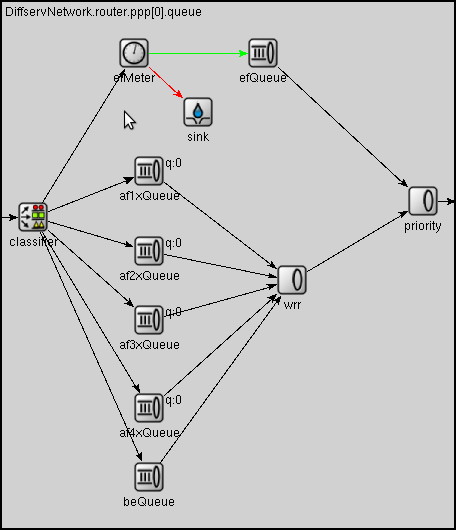
\includegraphics[scale=0.7]{figures/DiffservQueue.png}
\end{center}

The incoming packets are first classified according to
their DSCP field. DSCPs other than AFxy and EF are handled
as BE (best effort).

EF packets are stored in a dedicated queue, and served first
when a packet is requested. Because they can preempt the other
queues, the rate of the EF packets should be limited to a fraction
of the bandwith of the link. This is achieved by metering the EF
traffic with a token bucket meter and dropping packets that
does not conform to the traffic profile.

There are other queues for AFx classes and BE. The AFx queues
use RED to implement 3 different drop priorities within the class.
BE packets are stored in a drop tail queue.
Packets from AFxy and BE queues are sheduled by a WRR scheduler,
which ensures that the remaining bandwith is allocated among the classes
according to the specified weights.

%%% Local Variables:
%%% mode: latex
%%% TeX-master: "usman"
%%% End:



\cleardoublepage

\chapter{The MPLS Models}
\label{cha:mpls}


\section{Overview}

TODO


\section{MPLS/RSVP/LDP Model - Implemented Standards}

The implementation follows those RFCs below:

\begin{itemize}
  \item RFC 2702: Requirements for Traffic Engineering Over MPLS
  \item RFC 2205: Resource ReSerVation Protocol
  \item RFC 3031: Multiprotocol Label Switching Architecture
  \item RFC 3036: LDP Specification
  \item RFC 3209: RSVP-TE Extension to RSVP for LSP tunnels
  \item RFC 2205: RSVP Version 1 - Functional Specification
  \item RFC 2209: RSVP Message processing Version 1
\end{itemize}

\section{The MPLS Module}

TODO

\section{The LDP Module}

TODO

\section{LIB Table File Format}

The format of a LIB table file is:

The beginning of the file should begin with comments. Lines that begin with \# are treated
as comments. An empty line is required after the comments. The "LIB TABLE"
syntax must come next with an empty line. The column headers follow. This header
must be strictly "In-lbl In-intf Out-lbl Out-intf". Column
values are after that with space or tab for field separation.
The following is a sample of lib table file.

\begin{verbatim}
#lib table for MPLS network simulation test
#lib1.table for LSR1 - this is an edge router
#no incoming label for traffic from in-intf 0 &1 - LSR1 is ingress router for those traffic
#no outgoing label for traffic from in_intf 2 &3 - LSR 1 is egress router for those traffic

LIB TABLE:

In-lbl  In-intf         Out-lbl     Out-intf
1       193.233.7.90    1           193.231.7.21
2       193.243.2.1     0           193.243.2.3
\end{verbatim}


\section{The traffic.xml file}

The traffic.xml file is read by the RSVP-TE module (RSVP).
The file must be in the same folder as the executable
network simulation file.

The XML elements used in the "traffic.xml" file:

\begin{itemize}
  \item \ttt{<Traffic></Traffic>} is the root element. It may contain one or more \ttt{<Conn>} elements.
  \item \ttt{<Conn></Conn>} specifies an RSVP session. It may contain the following elements:
  \begin{itemize}
    \item \ttt{<src></src>} specifies sender IP address
    \item \ttt{<dest></dest>} specifies receiver IP address
    \item \ttt{<setupPri></setupPri>} specifies LSP setup priority
    \item \ttt{<holdingPri></holdingPri>} specifies LSP holding priority
    \item \ttt{<bandwidth></bandwidth>} specifies the requested BW.
    \item \ttt{<delay></delay>} specifies the requested delay.
    \item \ttt{<route></route>} specifies the explicit route. This is a comma-separated
      list of IP-address, hop-type pairs (also separated by comma).
      A hop type has a value of 1 if the hop is a loose hop and 0 otherwise.
  \end{itemize}
\end{itemize}

The following presents an example file:

\begin{verbatim}
<?xml version="1.0"?>
<!-- Example of traffic control file -->
<traffic>
   <conn>
       <src>10.0.0.1</src>
       <dest>10.0.1.2</dest>
       <setupPri>7</setupPri>
       <holdingPri>7</holdingPri>
       <bandwidth>400</bandwidth>
       <delay>5</delay>
   </conn>
   <conn>
       <src>11.0.0.1</src>
       <dest>11.0.1.2</dest>
       <setupPri>7</setupPri>
       <holdingPri>7</holdingPri>
       <bandwidth>100</bandwidth>
       <delay>5</delay>
   </conn>
</traffic>
\end{verbatim}

An example of using RSVP-TE as signaling protocol can be found in
ExplicitRouting folder distributed with the simulation. In this
example, a network similar to the network in LDP-MPLS example is
setup. Instead of using LDP, "signaling" parameter is set to 2 (value
of RSVP-TE handler). The following xml file is used for traffic
control. Note the explicit routes specified in the second connection.
It indicates that the route is a strict one since the values of every
hop types are 0. The route defined is 10.0.0.1 -> 1.0.0.1 ->
10.0.0.3 -> 1.0.0.4 -> 10.0.0.5 -> 10.0.1.2.

\begin{verbatim}
<?xml version="1.0"?>
<!-- Example of traffic control file -->
<traffic>
    <conn>
        <src>10.0.0.1</src>
        <dest>10.0.1.2</dest>
        <setupPri>7</setupPri>
        <holdingPri>7</holdingPri>
        <bandwidth>0</bandwidth>
        <delay>0</delay>
        <ER>false</ER>
    </conn>
    <conn>
        <src>11.0.0.1</src>
        <dest>11.0.1.2</dest>
        <setupPri>7</setupPri>
        <holdingPri>7</holdingPri>
        <bandwidth>0</bandwidth>
        <delay>0</delay>
        <ER>true</ER>
        <route>1.0.0.1,0,1.0.0.3,0,1.0.0.4,0,1.0.0.5,0,10.0.1.2,0</route>
    </conn>
</traffic>
\end{verbatim}

%%% Local Variables:
%%% mode: latex
%%% TeX-master: "usman"
%%% End:



\cleardoublepage

\chapter{Applications}
\label{cha:apps}

TODO

%%% Local Variables:
%%% mode: latex
%%% TeX-master: "usman"
%%% End:


\cleardoublepage

\bibliographystyle{alpha}
\bibliography{inet-developers-guide}


%% no need for the following since 'tocbibind' package
%% \phantomsection
%% \addcontentsline{toc}{chapter}{\indexname}
\printindex

\end{document}

%%% Local Variables:
%%% mode: latex
%%% TeX-master: t
%%% End:
